
In \autoref{ch:pl}, we considered the amount of information encoded in the spiking activity of a population of cortical neurons in both the \acf{V1} and visual area 4 (\acsu{V4}).
In this chapter, we will consider the population activity encoded in the \ac{CSD}, the distribution of flows of current within the cortex.
We examine the \ac{CSD} within \ac{V1} across the depth of a single cortical column, and decompose the signal into oscillations at different frequency ranges, examining the amount of information the power of the oscillations contain about a naturalistic video stimulus.


% =============================================================================
\section{Background}
% =============================================================================


% The cerebral cortex generates activity over a wide range of frequencies. Different frequencies are believed to have a different neural origin. In some cases different frequency ranges carry independent information about the stimuli. Different oscillations ranges seem to influence brain function, perception and regulate communication across neural populations. 


The aggregate population activity generates oscillations in the medium within which neurons reside.
These oscillations in the \acp{LFP} arise through rhythmic or correlated activity within the local population.
% This rhythmic activity may consist of spiking activity, but can also be sub-threshold, non-spiking, changes in the membrane potential across the local population.
The \ac{LFP} is believed to consist of various components, principally generated by synaptic input currents and their return currents, however there is also contribution from slow calcium-mediated spiking activity and even from fast sodium-mediated action potentials \citep{Einevoll2013}.
In particular, pyramidal neurons contribute more to the creation of \acp{LFP} than any other type of neuron.
This is due to their large dendritic trees, which result in a large spatial separation between synaptic inputs and return currents.
% When the \ac{LFP} is decomposed into different frequency bands, contribution amount of contribution from spiking activity depends on the frequency range considered.
\acp{LFP} are diffuse, with uncorrelated synaptic activity inducing changes in potential at a range of \SI{200}{\micro\metre}, whilst the effects of correlated activity can be seen at recording sites millimetres away from the source.
Since \acp{LFP} are generated by localised synaptic currents, it is often more useful to construct a model of the \acf{CSD} which underlies the observed potentials.
Furthermore, lower frequency components of the \ac{LFP} have larger spatial extent than high frequency components \citep{Leski2013}.
% One of the most keen applications of \ac{LFP} analysis is in brain-computer interfaces, since \ac{LFP} recordings reflect population activity and are more stable than recordings from individual neurons.

Many brain functions have been tied to cortical oscillations \citep{Buzsaki2004science,Einevoll2013,Colgin2016}, including sensory processing \citep{Henrie2005,Kreiman2006,Mazzoni2011,Szymanski2011}, motor function \citep{Scherberger2005,Rickert2005}, planning \citep{Buzsaki2015}, attention \citep{Fries2001,Jensen2007,Klimesch2012}, perception \citep{Grossberg1991,Fries1997,Gross2007}, memory \citep{Klimesch1999,Raghavachari2001,Pesaran2002,Jensen2002,Jensen2007,Liebe2012}, even stimulating microglia to reduce the plaque associated with Alzheimer's disease \citep{Iaccarino2016} and coupling of the brain to the gastric system \citep{Monto2008,Richter2017}.
In addition to this, theoretical research hypothesises that cortical oscillations gate the transfer of information between cortices \citep{Ahissar2015}, enable consciousness \citep{Llinas1998}, and facilitate predictive coding \citep{Arnal2012}, speech \citep{Giraud2012}, and working memory \citep{Dipoppa2013}.

In particular, previous work has demonstrated that in the macaque \ac{V1} there are two \ac{LFP} frequency bands, \SIrange{1}{8}{Hz} and \SIrange{60}{100}{Hz}, which encode independent information in the macaque \ac{V1} about natural stimuli \citep{Belitski2008}.
We hypothesised that the two frequency bands are generated through different cortical processes.
In this study, we investigated where within the cortical depth these frequency bands are most informative.
Under the hypothesis of two independent cortical circuits generating the two bands, we expect to observe that the two frequency bands are generated at different cortical depths.


% =============================================================================
\section{Methods}
\label{sec:lam_exp}
% =============================================================================

% \subsection{Ethics statement}

The experimental data analysed in this chapter was acquired by Daniel Zaldivar and Yusuke Murayama, under the supervision of Nikos Logothetis at the Max Plank Institute for Biological Cybernetics.
Data was collected from \ac{V1} in four healthy rhesus monkeys (Macaca mulatta; four males \SIrange{8}{11}{kg}; \SIrange{10}{12}{years}).
All the experimental procedures were approved by the local authorities (Regierungspr\"asidium, Baden-W\"urttemberg, T\"ubingen, Germany; Project Number KY4/09) and were in full compliance with the guidelines of the European Community (EUVD 86/609/EEC) and were in concordance with the recommendation of the Weatherall report for the care and use of non-human primates \citep{Weatherall2006}.
The animals were group-housed in an enriched environment, under daily veterinarian care.
Weight, food and water intake were carefully monitored on a daily basis.


\subsection{Anesthesia for neurophysiology}

The anesthesia protocol for all the experimental procedures have been described previously \citep{Logothetis1999,Logothetis2001}.
Briefly, glycopyrrolate (\SI{0.01}{mg.{kg}^{-1}}) and ketamine (\SI{15}{mg.{kg}^{-1}}), were used previous to general anesthesia.
Induction with fentanyl (\SI{3}{mg.{kg}^{-1}}), thiopental (\SI{5}{mg.{kg}^{-1}}) and succinylcholine chloride (\SI{3}{mg.{kg}^{-1}}), animals were intubated and ventilated using a Servo Ventilator 900C (Siemens, Germany) maintaining an end-tidal \ce{CO2} of \SIrange{33}{35}{mm.Hg} and oxygen saturation above \SI{95}{\percent}.

The anesthesia was maintained with remifentanil (\SIrange{0.5}{2}{\micro\gram.kg^{-1}.\min}) and mivacurium chloride (\SIrange{2}{6}{mg.kg^{-1}.h}) which ensured no eye movement during electrophygiological recordings.
The anesthetics dosage were established by measuring stress hormones and were selected to ensure unaffected physiological response at normal catecholamine concentrations \citep{Logothetis1999}.
In addition, it has been shown that using remifentanil has no significant effect on the neurovascular and neural activity of brain areas that do not belong to the pain matrix \citep{Goense2008,Zappe2008}.
In particular, visual cortex does not bind remifentanil.
We monitored the physiological state of the monkey continuously and kept within normal limits.
Body temperature was tightly maintained at \SIrange{38}{39}{\celsius}.
Throughout the experiment lactate Ringer's (Jonosteril, Fresenius Kabi, Germany) with \SI{2.5}{\percent} glucose was continuously infused at a rate of \SI{10}{ml.kg^{-1}.h^{-1}} in order to maintain an adequate acid-base balance and intravascular volume and blood pressure were maintained by the administration of hydroxyethyl starch as needed (Volulyte, Fresenius Kabi, Germany).

We used anesthetised animals as it allows for a longer data acquisition for each session, and lets us associate the neural activity to specific features of the stimulus without the effects of the animal's cognitive state, including effects of attention and arousal.
Such phenomena would introduce additional signals, complicating the interpretation of the results.


\subsection{Visual stimulation}

A few drops of \SI{1}{\percent} cyclopentolate hydrochloride were used in each eye to achieve mydriasis.
Animals were wearing hard contact lenses (W\"ohlk-Contact-Linsen, Sch\"onkirchen, Germany) to focus the eyes on the stimulus plane.
The visual stimulation in all experimental sessions was presented to the eye for which the recording sites had the stronger ocular preference.
The stimulus was presented using either an in-house custom-built projector (SVGA fibre-optic system with a resolution of \num{800x600} pixels, a frame rate of \SI{30}{Hz}), or a \ac{CRT} monitor (Iiyama MA203DT Vision Master Pro 513, frame rate \SI{118}{Hz}) placed at eye level, \SI{50}{\centi\metre} in front of the eye.
We found the same results with both display devices, except that when using a monitor refresh of \SI{30}{Hz} the stimulus induced cortical oscillations at \SI{30}{Hz} not seen otherwise.
Since this is the result of using an artificial stimulus with a low refresh rate (a well-known issue at this stimulus frequency), we removed this from the data (see \autoref{sec:lam_artefact}) and pooled the results across all sessions.
The visual stimulus consisted of high contrast (\SI{100}{\percent}), gamma corrected, fast-moving, colourful movie clips (no soundtrack) from a commercially available movie.
Stimulus timings were controlled by a computer running a real-time OS (QNX, Ottawa, Canada).
Stimulus-on periods of \SI{120}{\second} (\num{5} sessions; \num{1} session: \SI{40}{\second}) were interleaved with stimulus-off periods (isoluminant grey screen) of \SI{30}{\second}.


\subsection{Luminosity function}
\label{sec:lam_lumos}

In order to best approximate the luminosity perceived by macaques, we relied on analogies with the human visual system.
Research in humans suggests the luminosity function is linearly related to the L- and M-cone activation, and independent of the S-cone activation \citep{Stockman2008}.
Furthermore, the weighting of L and M activations towards perceived luminance is believed to be similar to the L:M ratio in the individual \citep{Stockman2008}.
Old world monkeys such as macaques have an L:M ratio which is approximately 1:1 \citep{Dobkins2000}, so we assumed a luminosity function equally weighed between the L and M cone activations, $Y(f) = L(f) + M(f)$.
The \SI{10}{\degree} cone fundamentals%
\footnote{The cone fundamentals are similar to the pigment response curves shown in \autoref{fig:bg_cone_responses}, but account for the non-linear relationship between the changes in the pigment and the response produced by the cone.}
of \citet{Stockman2000} were used%
\footnote{Tabulated in CSV format by the Colour \& Vision Research Laboratory of University College London, \url{http://www.cvrl.org/cones.htm}.}
since the cone fundamentals of old world monkeys are known to be very similar to humans \citep{Dobkins2000}.
We recorded the emission spectra for both our display devices with a light-spectrometer.
By taking the product of the emission spectra for pure red, green and blue with the luminosity function, integrating over wavelength and normalising, we obtained the relative luminance in terms of pixel intensity for the two devices used in the experiment,
\begin{align}
Y_{\text{projector}} &= 0.2171 \cdot R + 0.6531 \cdot G + 0.1298 \cdot B\\
Y_{\text{CRT}}       &= 0.1487 \cdot R + 0.6822 \cdot G + 0.1691 \cdot B
.\end{align}
Here, $R$, $G$, and $B$ denote the fractional pixel intensity in the movie file.

\subsection{Neurophysiology data collection}

The electrophysiological recordings were performed by doing a small skull trepanation, after which the dura was visualised with a microscope (Zeiss Opmi MDU/S5, Germany) and carefully dissected.
The electrodes were slowly advanced into the visual areas under visual and auditory guidance using manual micromanipulator (Narashige Group, Japan).
Electrodes consisted of laminar probes (NeuroNexus Technologies, Ann Arbor, USA).
These electrodes contained \num{16} contacts on a single shank \SI{3}{\milli\metre} long and \SI{150}{\micro\metre} thick.
The electrode sites were spaced at \SI{150}{\micro\metre} apart, with a recording area of \SI{413}{\micro\metre^2} each.
We used a flattened silver wire, which was positioned under the skin, as reference electrode \citep{Murayama2010}.
The recording access was filed with a mixture of \SI{0.6}{\percent} agar dissolved in \ac{NaCl} \SI{0.9}{\percent}, pH 7.4 solution which guaranteed good electrical connection between the ground contact and the animal \citep{Oeltermann2007760}.
The impedance of the contact points was measured during the experiments and ranged from \SIrange{480}{800}{\kilo\ohm}.
The signals were amplified and filtered into a broadband of \SIrange{1}{8000}{Hz} (Alpha-Omega Engineering, Nazareth, Israel) and then digitised at \SI{20.833}{\kilo\Hz} with \SI{16}{bit} resolution (PCI-6052E; National Instruments, Austin, TX).


\acused{CRT}
\begin{table}[htbp]
\small
\centerline{
\begin{tabular}{l l m{1.05cm} m{1cm} r r}
\toprule
Session &
    Display &
        Frame rate (\si{fps}) &
            Freq. Removed (\si{Hz}) &
                Eccentricity &
                    Stimulus size\\
\midrule
\sesname{E07nm1} &
    \ac{CRT} &
        \raggedleft \num{118.089} &
            \num{50}, \num{150} &
                \SI{4.8\pm3.0}{\degree} &
                    \SI{17.9 x 13.5}{\degree}\\
\sesname{F10nm1} &
    Projector &
        \raggedleft \num{30.015} &
            \num{30}, \num{60} &
                \SI{2.7\pm1.0}{\degree} &
                    \SI{15.0 x 11.3}{\degree}\\
\sesname{H05391} &
    Projector &
        \raggedleft \num{30.015} &
            \num{30} &
                \SI{7.7\pm1.0}{\degree} &
                    \SI{20.0 x 15.0}{\degree}\\
\sesname{H05nm7} &
    Projector &
        \raggedleft \num{30.015} &
            \num{30}, \num{60} &
                \SI{4.2\pm1.0}{\degree} &
                    \SI{15.0 x 11.3}{\degree}\\
\sesname{H05nm9} &
    \ac{CRT} &
        \raggedleft \num{118.089} &
            ~ &
                \SI{4.0\pm3.0}{\degree} &
                    \SI{18.0 x 13.4}{\degree}\\
\sesname{J10nm1} &
    \ac{CRT} &
        \raggedleft \num{118.089} &
            ~ &
                \SI{2.6\pm3.0}{\degree} &
                    \SI{17.9 x 13.4}{\degree}\\
\bottomrule
\end{tabular}
}
\caption{
\captionemph{Metadata for recording sessions.}
Stimuli were presented using either an in-house custom-built projector (SVGA fibre-optic system with a resolution of \num{800x600} pixels; ``Projector''), or a cathode ray tube monitor (Iiyama MA203DT Vision Master Pro 513; ``\ac{CRT}'') placed at eye level, \SI{50}{\centi\metre} in front of the eye.
Videos presented at \SI{118}{Hz} were up-sampled versions of the original \SI{30}{Hz} video, which was achieved by repeating each frame four times.
For artefact removal methodology, see \autoref{sec:lam_artefact}.
}
\label{tab:lam_md}
\end{table}


\subsection{Artefact removal}
\label{sec:lam_artefact}

An artefact removal procedure was performed to reduce the effects of line noise (one session) and phase locking to the refresh rate of the stimulus (the three sessions with \SI{30}{Hz} stimulus).
Artefact frequencies (see \autoref{tab:lam_md}) were identified by large, localised peaks in the power spectral density, which was computed with the periodogram method.
In each case, the average artefact waveform was found and subtracted from the recorded signal.
To correct for phase shifts of the artefact, the averaging and subsequent subtraction were performed in blocks of \num{50} artefact periods with a phase chosen to maximise the cross-covariance of the signal with the artefact waveform.


\subsection{Current source density}
\label{sec:lam_csd}

The \ac{CSD} was derived from the \ac{LFP} using the inverse \ac{CSD} method \citep{Pettersen2006}.
To compute this, we used a $\delta$-source model of local field generation, in which the cortical column is approximated by a finite set of infinitely thin discs (one for each recording site).
We used a diameter of \SI{500}{\micro\metre}, chosen to correspond to the effective size of columnar activity \citep{Horton2005,Lund2003}.
Since this method requires an even spacing between voltage measurements, gaps caused by faulty recording contacts in the electrode were filled in with a local average \citep{Wojcik2010}.
A homogeneous cortical conductivity of \SI{0.4}{\siemens\per\metre} was assumed \citep{Logothetis2007}.
The agar solution placed on top of the recording access point had an \ac{NaCl} concentration of \SI{9}{\mg\per\mL}, and the conductivity of this was estimated to be \SI{2.2}{\siemens\per\metre} \citep{Kandadai2012}.
The \ac{CSD} was spatially smoothed with a three-point Hamming filter.


\subsection{Multi-unit activity}

% \autoref{fig:lam_1}:~\ac{MUA} was calculated by band-passing the voltage recording between \SIrange{900}{3000}{Hz} with a zero-phase sixth-order Butterworth filter, taking the absolute value, applying a \SI{300}{Hz} low pass third-order Butterworth filter, and then downsampling.
% This yields a smoothed spike rate, analogous to a population firing rate.

The \ac{MUA} was calculated by downsampling the raw signal by a factor of \num{3}, band-passing the voltage recording between \SIrange{900}{3000}{Hz} with a zero-phase sixth-order \ac{IIR} Butterworth filter, taking the absolute value, and then downsampling by a further factor of \num{12}.


\subsection{Receptive field locations}
\label{sec:lam_rf}

The spatial \acp{RF} were found by reverse correlating the \ac{MUA} and the pixel-by-pixel Z-scored frame-by-frame difference in luminance with an assumed latency of \SI{66.7}{\milli\second}.
The rate of change in luminance was used because it is known to correlate well with thalamic drive.
For each session, the \ac{RF} centre was manually located using the average of the reverse correlation score across all cortical channels such that the centre was near the point with maximum reverse correlation and the region with highest correlation fell within \SI{1}{\degree} of the \ac{RF} centre.


% \subsubsection{Nuclear magnetic resonance data collection}
%
% For two of the four monkeys involved in the study, we made use of high-resolution \ac{NMR} anatomical scans (collected for a different experiment) to measure the cortical thickness at the recording site used (\autoref{fig:lam_nmr_e07} and \autoref{fig:lam_nmr_h05}).
%
% To estimate the cortical thickness at the recording site of the laminar electrodes, high-resolution \ac{NMR} anatomical scans were acquired at the vertical using a \SI{7}{T} scanner with a \SI{60}{\centi\metre} diameter bore (Bruker BioSpin GmbH, Ettlingen, Germany).
% A custom-made chair was used to position the monkey in the magnet.
% We used a single-shot gradient \ac{EPI} with a \ac{FOV} of \SI{96x96}{\milli\metre} and matrix of \num{256x256}.
% We acquired 18 a thickness of \SI{1}{\milli\metre}, TE/TR 15/\SI{2000}{\milli\second} and flip angle of \SI{90}{\degree}.
%
% Animal \sesname{H05} was found to have a cortical thickness of \SI{\sim 1.7}{mm} at the recording site, whilst \sesname{E07} had a thickness of \SI{\sim 1.56}{mm}.
%
% The thickness of cortical material included in the \ac{SG}, \ac{G} and \ac{IG} components is \SI{\sim 0.3}{mm} more than the measured obtained from the \ac{NMR} recordings.
% We believe this discrepancy is due to the inflammation of the cortex in response to the trauma of the electrode penetration and the non-perpendicularity of the electrode penetration angle.


\subsection{Aligning electrode penetrations}
\label{sec:lam_align}

\let\truelinewidth\linewidth

For each recording session, the electrode was implanted in \ac{V1} at the recording site.
% indicated in \autoref{fig:lam_nmr_e07} and \autoref{fig:lam_nmr_h05}.
For each penetration, we endeavoured to align the electrode such that the most shallow electrode contact was at the boundary between cortical matter and the dura (near \aclu{L1}; \acs{L1}).
However, this \textit{ad-hoc} method of alignment is unreliable, in part due to variation in cortical and laminar thickness both within and between subjects.
Therefore, we performed \textit{post-hoc} realignment of the electrode contacts using the same methodology as \citet{Self2013} and \citet{VanKerkoerle2014}, described below.

\begin{sidewaysfigure}
%     \subfloat[][\acs{NMR} cross-section of \sesname{E07}'s brain.\label{fig:lam_nmr_e07}]{%
%         \includegraphics[scale=.5]{%
% figs/recordings/fig1S2-amended-E07.eps}}
%     \hspace*{\fill}\hspace{.2cm}\hspace*{\fill}
%     \subfloat[][\acs{NMR} cross-section of \sesname{H05}'s brain.\label{fig:lam_nmr_h05}]{%
%         \includegraphics[scale=.5]{%
% figs/recordings/fig1S2-amended-H05.eps}}
%     \hspace*{\fill}
%     \\

    \hspace{1.25cm}
    \subfloat[][Alignment of \acs{CSD} across sessions.\label{fig:lam_align_csd}]{%
        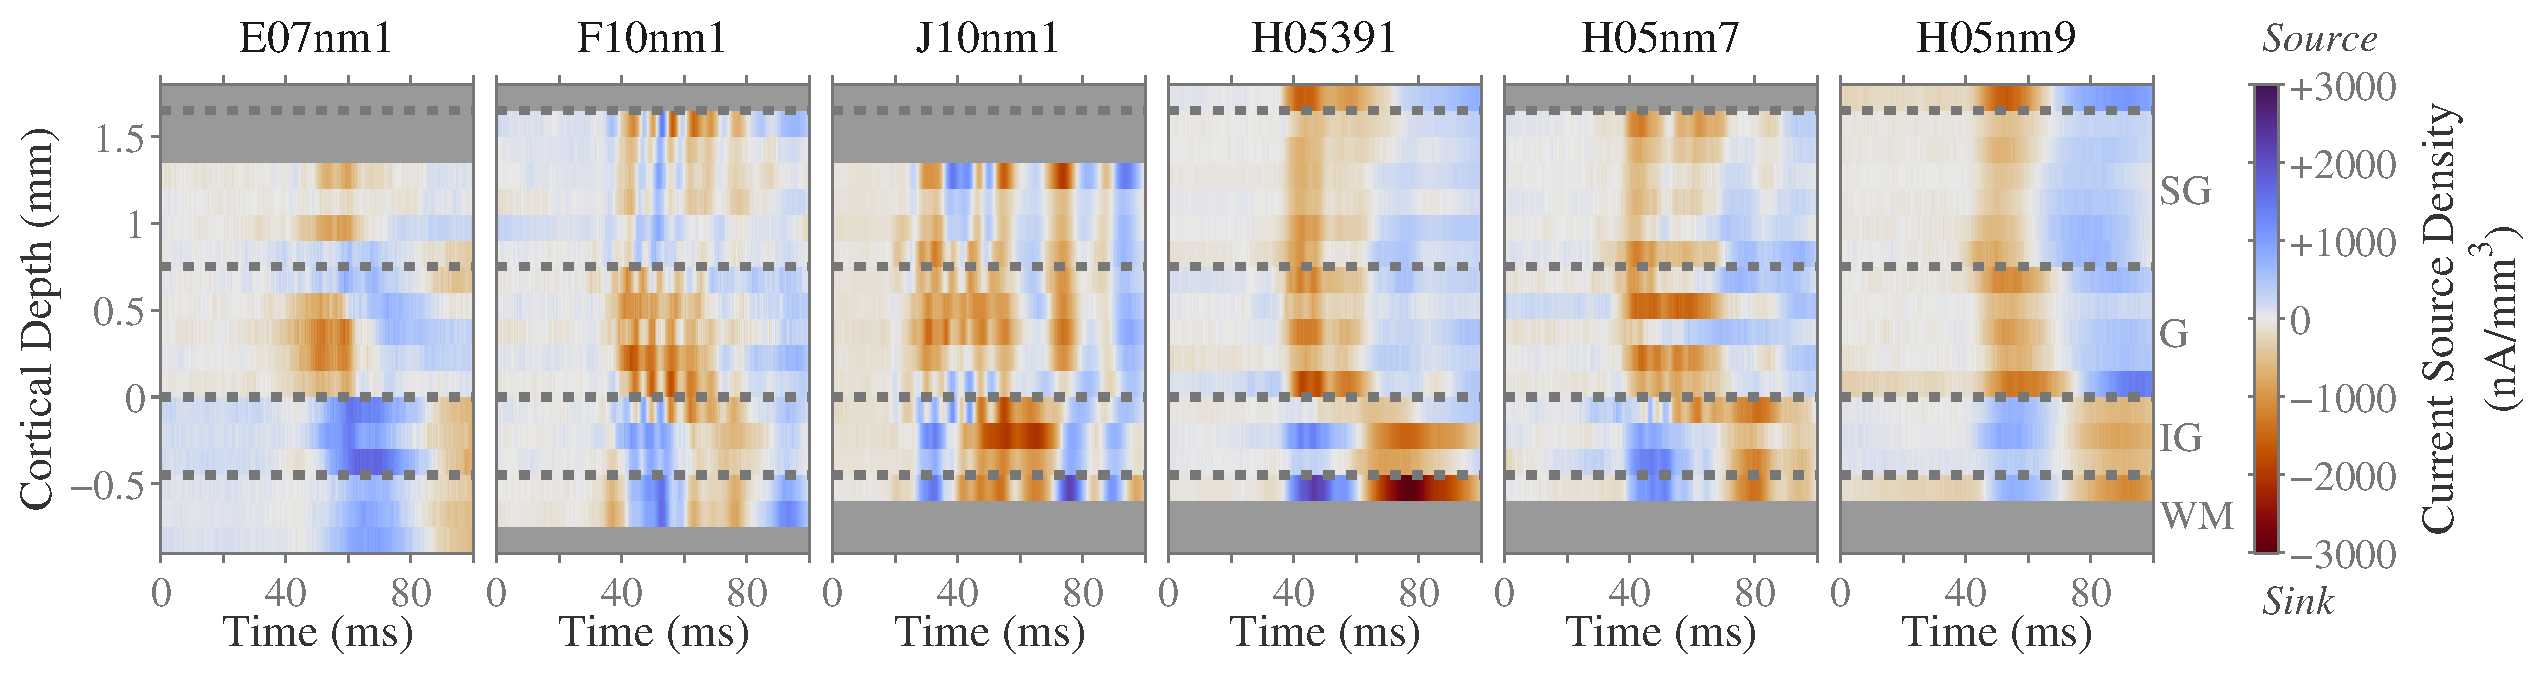
\includegraphics[scale=.35]{%
figs/recordings/sigtrlavg-allsestb-6ses-photodiode-mixed-Cln-none-none-mean-iCSD-b0=none-0.eps}
}

    \hspace{1.25cm}
    \subfloat[][Alignment of \acs{MUA} across sessions.\label{fig:lam_align_mua}]{%
        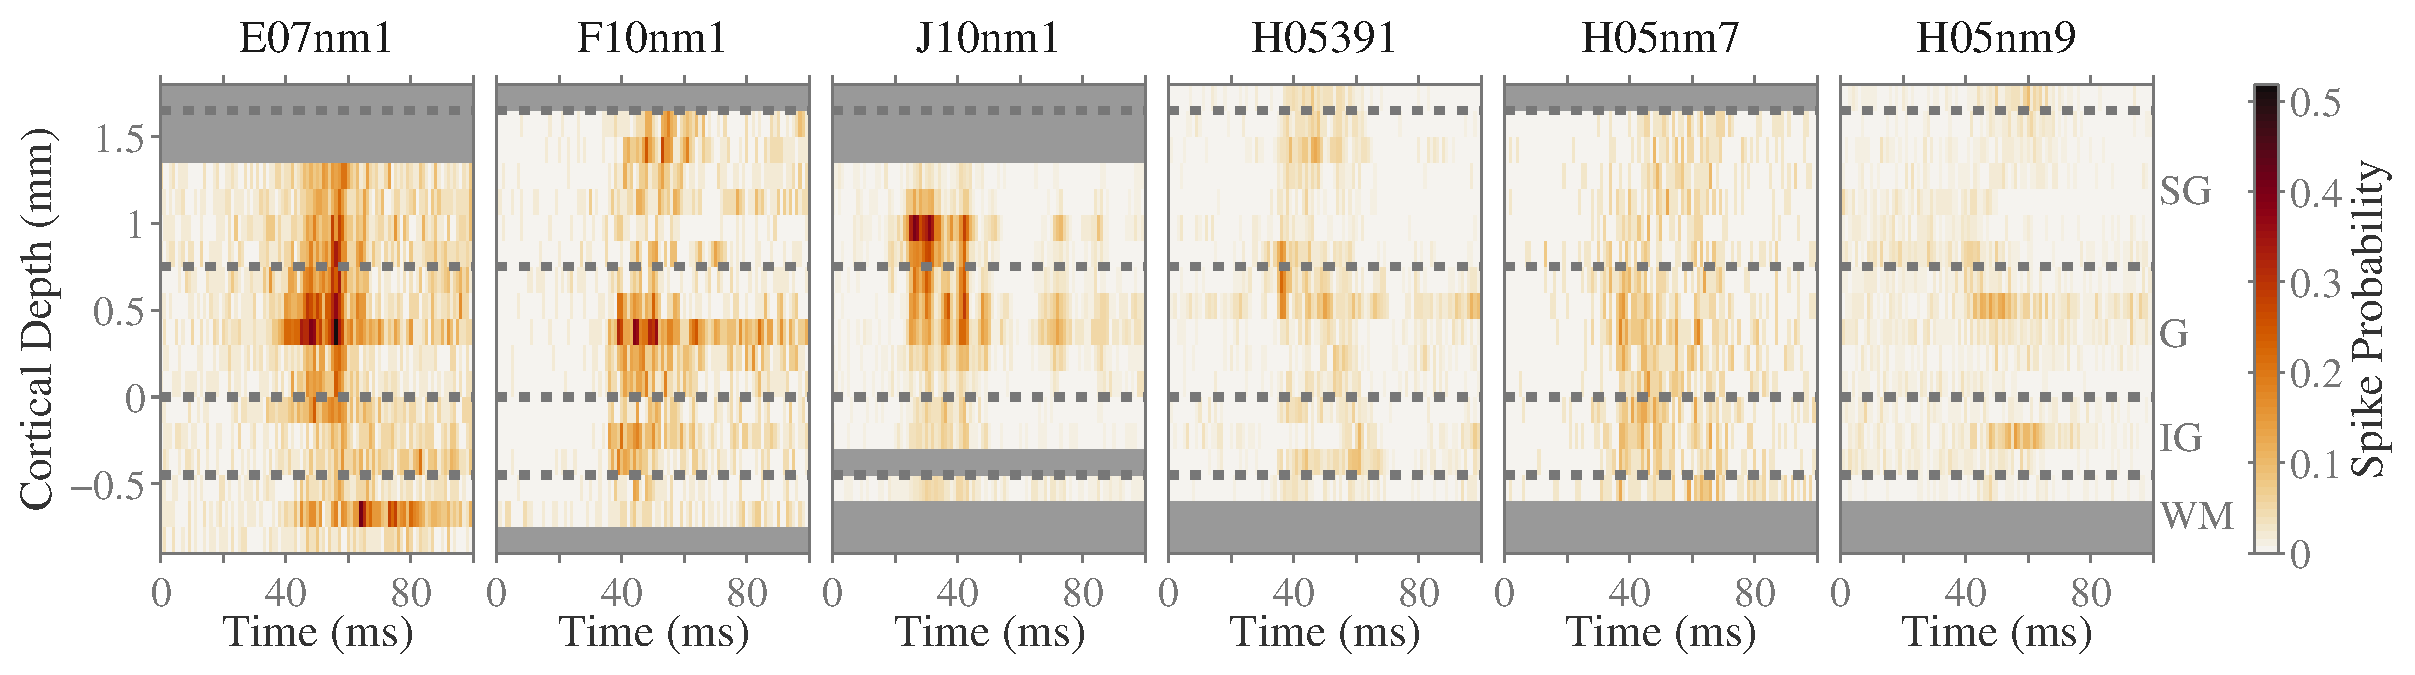
\includegraphics[scale=.35]{%
figs/recordings/sigtrlavg-allsestb-6ses-photodiode-mixed-Spkt-none-none-mean-0.eps}
}

\centering \begin{minipage}{15cm}
\caption{
\captionemph{Electrode alignment.}
% \protect\subref{fig:lam_nmr_e07} and \protect\subref{fig:lam_nmr_h05}:~High resolution \ac{NMR} scans of two animals used to measure cortical thickness.
\protect\subref{fig:lam_align_csd}:~Stimulus triggered average \ac{CSD} responses, post-alignment.
For sessions \sesname{H05391}, \sesname{H05nm7}, \sesname{H05nm9} and \sesname{E07nm1}, the average response to onset of the movie stimulus is shown, whereas for sessions \sesname{F10nm1} and \sesname{J10nm1} the response to a full-field flash is shown.
\protect\subref{fig:lam_align_mua}:~Corresponding spike densities for the responses in panel \protect\subref{fig:lam_align_csd} (\SI{1}{\milli\second} window duration).
}
\end{minipage}
\label{fig:lam_s1}
%
\end{sidewaysfigure}

To identify the depth of each electrode contact, we measured the potential evoked in response to the onset of the movie clip, and in response to full-screen maximum-luminance \SI{100}{\milli\second} flash stimuli with \SI{6}{\second} intervals.
From the measured potentials, we identified the boundary between the \ac{G} and \ac{IG} compartments as the source-sink reversal in the evoked \ac{CSD} \citep{Mitzdorf1979,Mitzdorf1985}.
For this measurement, the \ac{CSD} was computed from the \ac{LFP} as described in \autoref{sec:lam_csd}, but without applying the Hamming filter to spatially smooth the signal.
The data from each electrode was re-aligned such that the source-sink reversal for each recording session was at a depth of \SI{0}{\milli\metre}, as shown in \autoref{fig:lam_align_csd}.
We estimated the location of the boundary between the \ac{G} and \ac{SG} compartments by cross-referencing literature describing the average thickness of cortical laminae in Macaca mulatta, area 17 \citep{Lund1973,OKusky1982}.

The majority of thalamic afferents in \ac{V1} stimulate \ac{L4} (though some argue the connection is indirect; \citealp{Hansen2012}), and studies have found the first cortical response to the onset of stimuli is at \acsu{L4Ca}, in the middle of the \ac{G} compartment \citep{Callaway1998}.
Consequently, we also extracted spikes from the broadband recordings, and investigated the spatiotemporal distribution of the spiking response to the onset of the stimulus.
For this purpose, we extracted spikes by first high-pass filtering the raw signal above \SI{500}{Hz} with a zero-phase eighth-order \ac{IIR} Butterworth filter.
We classified any points more than \num{3.5} standard deviations above the mean signal during inter-stimulus periods as a spike, under the restriction of a minimum inter-spike-interval of \SI{1}{\milli\second}.
Finally, we binned the spikes in intervals of \SI{1}{\milli\second} and took the average count over all stimulus presentations to find the instantaneous spike probability.
As shown in \autoref{fig:lam_align_mua}, there is a strong and early response near the middle of \ac{G} across all recording sessions, indicating the electrode alignment is correct.


\subsection{Power as a function of depth and frequency}
\label{sec:lam_power_method}

To derive the power as a function of temporal frequency, the cortical data (\ac{LFP} and \ac{CSD}) was filtered in a series of bands each with a fractional bandwidth of \SI{50}{\percent}.
We held the fractional bandwidth constant instead of the actual bandwidth because cortical power falls off rapidly with frequency, approximately following a power law.
Each successive band we considered begins and ends with frequencies \num{1.291} times higher than the last, so that each band has \SI{0}{\percent} overlap with bands further away than its immediate neighbours and a \SI{44}{\percent} and \SI{56}{\percent} overlap with its preceding and succeeding bands respectively.
The data was filtered with a zero-phase sixth-order \ac{IIR} Butterworth filter, after which the instantaneous power was estimated by taking the squared absolute value of the Hilbert transform.
The power in each band was integrated over a series of \SI{50}{\milli\second} windows, centred at the time of each frame change in the movie (once every \SI{33}{\milli\second}, leading to a \SI{50}{\percent} overlap of neighbouring windows).
The power in the \SIrange{4}{16}{Hz} and \SIrange{60}{170}{Hz} bands was extracted in the same manner.
In Figures \ref{fig:lam_power_lfp} and \ref{fig:lam_power_csd}, the average power over all frame presentations is shown, expressed in decibels relative to the average broadband \SIrange{1.5}{248}{Hz} power (estimated by summing the power in alternate bands of \SI{50}{\percent} fractional bandwidth).
Note that in Figures \ref{fig:lam_info} and \ref{fig:lam_info_sessions}, datapoints are shown at the band centres, identified as the arithmetic mean between the cutoff frequencies.


\subsection{Information as a function of depth and frequency}
\label{sec:lam_info_method}

Power in each band was computed as described in \autoref{sec:lam_power_method}.
Then, for each frequency band and depth, we took a \num{10}-bin histogram over the set of measured powers across all frame stimuli and repetitions, with the bin edges chosen such that \SI{10}{\percent} of the distribution fell into each bin.
We say that the power of the oscillation in a given frequency band is the \termemph{response} to the current frame on screen (the \termemph{stimulus}).
The \termemph{binned response} is then the identity of the bin within which the response (power) fell for the histogram.
The probability distribution of cortical power differs depending on which frame was presented.

We found the mutual information between the response and the stimulus (\autoref{eq:shannon-information}) using the \textpackage{Information Breakdown Toolbox} for MATLAB \citep{Magri2009}.
Bias in the estimated mutual information due to undersampling, described in \autoref{sec:info-bias}, was corrected for using the \ac{PT} method \citep{Treves1995}.
Each information calculation was also bootstrapped \num{20} times with a randomly shuffled mapping from stimulus to response (each also bias-corrected using \ac{PT}).
To ensure the amount of information was statistically significant, we checked each information estimate exceeded the bootstrap mean by more than \num{3} standard deviations of the bootstrap values.
The bootstrap mean was then subtracted from the estimated information, to counter any residual bias.


\subsection{Cortical distribution of power}

For each session, the distribution of power across the cortical depth (Figures \ref{fig:lam_power_lfp} and \ref{fig:lam_power_csd}, right-hand insets) was determined by normalising the power at each depth by the summed power across all cortical depths for that band.
We then took an average across sessions, weighted by the number of cortical recording sites in each session to prevent faulty (omitted) electrode contact sites from distorting the result.


\subsection{Information redundancy}
\label{sec:lam_redundancy_method}

Information redundancy was computed with the same stimuli and response powers as described above in \autoref{sec:lam_info_method}.
However, when computing the information redundancy we instead used \num{3} bins for the cortical response, with each histogram bin containing a third of the power datapoints across all repetitions of the movie stimulus.

First let us define $S$, to denote the set of stimuli, and $X$ and $Y$, two different responses (either different frequency bands or the same frequency bands but measured at different depths).
The information about the stimulus which is contained in each is $\I(X;S)$ and $\I(Y;S)$, which we computed using the methodology of \autoref{sec:lam_info_method}.
Additionally, we can consider the information in the joint distribution of simultaneously observed $X$ and $Y$ values, $\I(\left\{X,Y\right\};S)$.
To compute this value, we considered each combination of the pre-binned $X$ and $Y$ values as a different response, yielding a total of \num{9} different responses for $\{X,Y\}$.

Using this, we can derive the relative redundancy, which we define as
\begin{equation}
\label{eq:redundancy}
\operatorname{Redundancy}(X,Y;S)=\frac{
\I\left(X;S\right) + \I\left(Y;S\right) - \I\left(\left\{X,Y\right\};S\right)
}{
\I\left(\left\{X,Y\right\};S\right)
}
.\end{equation}
If $\operatorname{Redundancy}\left(X,Y;S\right) > 0$, this implies that $X$ and $Y$ contain redundant information about $S$.
If $\operatorname{Redundancy}\left(X,Y;S\right) < 0$, then $X$ and $Y$ are synergistic, such that knowing the paired state of $X$ and $Y$ simultaneously contains more information about $S$ than one would expect from the information just contained in $X$ and $Y$ individually.%
\footnote{%
\label{foot:redundancy_synergy}%
Unfortunately, since redundant and synergistic information co-occur when transitioning from knowing either $X$ or $Y$ to knowing their joint state ${X,Y}$, it is not possible to quantify the redundancy and synergy in isolation \citep{Latham2005,Averbeck2006,Williams2010,Griffith2014,Banerjee2015}.
The term which we refer to as ``Redundancy'' in \autoref{eq:redundancy}, is in reality the difference of the true (but unobservable) redundancy and synergy about $S$ in $X$ and $Y$.
Consequently, we can only conclude how much more redundancy than synergy there is, and when redundancy exceeds synergy that there is at least some redundancy.
For instance, in the case $\operatorname{Redundancy}\left(X,Y;S\right) = 0$, we can only conclude that there is the same amount of synergy as redundancy; it is not necessarily the case that $X$ and $Y$ contain exclusively independent information about $S$.
}

Additionally, we define the relative information gain as
\begin{equation}
\label{eq:infogain}
\operatorname{InfoGain}\left(Y\to\left\{X,Y\right\};S\right)=\frac{
\I\left(\left\{X,Y\right\};S\right) - \I\left(Y;S\right)
}{
\I\left(X;S\right)
},
\end{equation}
which is the amount of information gained about the stimulus when we already know $Y$ and $X$ is revealed to us, relative to the total amount of information about the stimulus contained in $X$.
$\operatorname{InfoGain}$ is an asymmetric measure, unlike $\operatorname{Redundancy}$.
If $X$ contains no more information about $S$ than is already contained in $Y$, then
$\I\left(\left\{X,Y\right\};S\right) = \I\left(Y;S\right)$
and we therefore have
$\operatorname{InfoGain}\left(Y\to\left\{X,Y\right\};S\right)=0$,
which makes intuitive sense in line with the concept of information gain.
However, if $\I\left(X;S\right)=0$, meaning $X$ contains no information about the stimulus, this would be divergent, so we instead choose to define
$\operatorname{InfoGain}\left(Y\to\left\{X,Y\right\};S\right)=0$
for this case.
If $X$ and $Y$ contain independent information about the stimulus,
$\I\left(\left\{X,Y\right\};S\right) = \I\left(X;S\right) + \I\left(Y;S\right)$,
then we find%
\footnote{
However, as stated above in \hyperref[foot:redundancy_synergy]{Footnote~\ref{foot:redundancy_synergy}},
$\operatorname{InfoGain} = 1$
is necessary but insufficient to conclude that $X$ and $Y$ contain exclusively independent information about $S$, since the same result can be achieved provided their synergy and redundancy effects cancel each other out.
Should $X$ and $Y$ contain more synergistic than redundant information about $S$, we will observe a relative information gain exceeding $1 = 100\%$.
}
that
$
\operatorname{InfoGain}\left(Y\to\left\{X,Y\right\};S\right) = 1 = 100\%
$.


\subsection{Signal and noise correlations}

We also computed the signal and noise correlation between pairs of unbinned responses to the movie stimulus.
The power was extracted as described in \autoref{sec:lam_power_method}.

For the signal correlation, the power in response to each stimulus was averaged over repetitions, producing a single mean response to each frame.
Then, for a given frequency band and recording depth, we correlated the average frame responses against the average responses elicited by another frequency band or depth using the Pearson correlation coefficient.

The noise correlation was computed by considering the power elicited during a single frame over all repetitions of the movie stimulus.
We then computed the Pearson correlation coefficient between responses $X$ and $Y$ over presentations of the same stimulus.
This was repeated for each pair of frames, and we took the average over all pairs as the noise correlation between $X$ and $Y$.

For both the signal and the noise correlation, we produced \num{20} bootstrap correlations by repeating the procedure for randomly paired responses by shuffling over either stimuli (signal) or repetitions (noise).
After averaging over sessions, correlation coefficients which were less than three standard deviations of the bootstraps from the bootstrap mean were deemed not significantly correlated (shown in white in Figures \ref{fig:lam_cxfrq_cor} and \ref{fig:lam_cxchn_cor}).


\subsection{Information about scene changes}
\label{sec:lam_scnchg_method}

To compute the amount of information encoded in the cortical activity about scene changes in the stimulus, we used the same procedure as described in \autoref{sec:lam_info_method}.
However, instead of computing the amount of information encoded about the unique identity of each frame in the movie stimulus, we labelled our stimuli as the number of frames since the last scene cut in the movie --- except for frames occurring more than $T_\text{sc}$ seconds after a scene cut which were instead all labelled as \num{-1}.
The parameter $T_\text{sc}$ was varied over the range $[0, 0.5]$.
This stimulus relabelling scheme meant that all frames following a scene cut were identified as the same stimulus condition, and frames not involved in a scene cut were labelled as another stimulus.

For this to provide a different quantification of information than labelling each individual frame with a unique ID, it is important that the number of collisions provided by the non-injective label remapping is sufficiently large.
Of the \num{96} scenes in the presented movie stimulus, only \num{5} had a duration shorter than \SI{0.5}{\second}, and all of these were at least \SI{0.4}{\second} long.
Consequently, when we chose $T_\text{sc} <= 0.4$, this encoding of the stimulus preserves information about the occurrence of a scene cut but all the information about which scene begins or its contents is removed.

For this part of the analysis, we did not integrate the power over \SI{50}{\milli\second} but instead used the instantaneous power as the cortical response.
We expressed the information about scene changes as a percentage of the total information present in the instantaneous \ac{CSD} power.


\subsection{Information about spatial components}
\label{sec:lam_spares_method}

To extract a measure of change in the movie at different spatial scales, we followed the procedure illustrated in \autoref{fig:lam_spares_method} and described below.
First, we took the two-dimensional fast-Fourier transform of a \SI{224}{px} square from the luminance of the movie (with luminance determined as described in \autoref{sec:lam_lumos}).
We applied a fourth-order \ac{IIR} Butterworth filter with a width of one octave by means of a mask in the Fourier domain, and then projected the output back to the spatial domain.
We then took the pixel-wise difference between each spatially-filtered pair of consecutive frames.
We integrated the absolute magnitude of the rate-of-change of spatially filtered luminance within a \SI{2}{\degree} diameter circular window centred at the receptive field location (determined as described in \autoref{sec:lam_rf}).

\begin{figure}[htbp]
% \centerline{
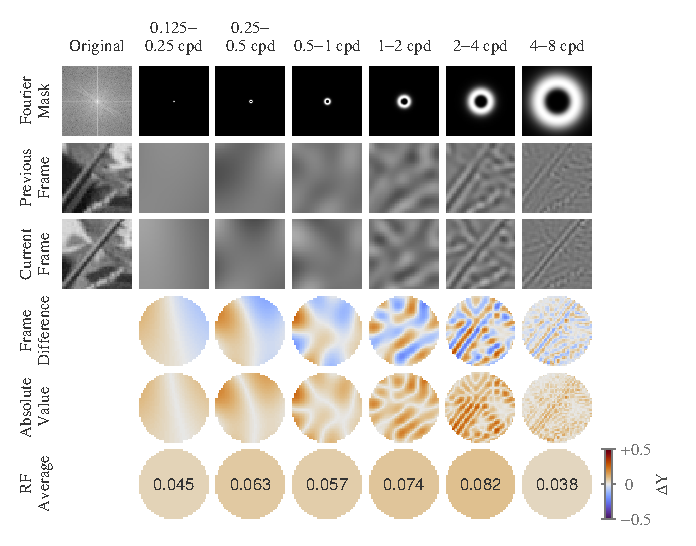
\includegraphics[width=1.05\linewidth]{paperfigs/fig4.eps}
% }
%
\caption{
\captionemph{Extraction of spatially filtered luminance components.}
The luminance of the original video (left) is fast-Fourier transformed in a \SI{224x224}{px} square for each frame (top-left: \ac{FFT} of  ``current frame'').
The mask isolates bands of spatial frequencies that are one octave wide (Row 1), yielding the spatially filtered frames (Rows 2 and 3).
The stimulus magnitude at each spatial frequency band was obtained by taking the luminance difference of successive frames (Row 4), taking its absolute value (Row 5), and averaging this within the receptive field (Row 6).
%This provides us with a temporal sequence of the rate of change of luminance for 
%each spatial resolution.
}%
\label{fig:lam_spares_method}
%
\end{figure}

Applying this to the entire movie provided a temporal sequence of luminance changes in each spatial range.
Similar to how the cortical response was binned, for each spatial range we took a \num{10}-bin histogram and labelled each frame according to the identity of the bin in which its rate-of-change of luminance fell.
The mutual information between this labelling of the stimulus and the neural response --- the power within \SIrange{4}{16}{Hz} and \SIrange{60}{170}{Hz} frequency bands --- was computed with a \SI{67}{\milli\second} lag between stimulus and response.


\subsection{Information about fine and coarse luminance changes}

Coarse and fine luminance changes in the stimulus were extracted using the methodology of \autoref{sec:lam_spares_method}, but instead of a bandpass filter we used a low-pass (\SI{<0.3}{\cpd}) and high-pass (\SI{>1}{\cpd}) fourth-order \ac{IIR} Butterworth filter respectively.
For both the \SIrange{4}{16}{Hz} and \SIrange{60}{170}{Hz} \ac{CSD} powers, we computed the correlation with and information about the coarse and fine luminance changes.


\subsection{Information latency between granular and infragranular compartments}
\label{sec:lam_latency_method}

The information about fine and coarse stimuli contained in \SIrange{4}{16}{Hz} and \SIrange{60}{170}{Hz} neural frequency bands was computed as a function of the lag between stimulus and response, in steps of \SI{1.73}{\milli\second}.
For each cortical recording depth, we determined the latency of the response as the lag which gave the maximum amount of information about the stimulus.
This step was performed for each session individually.
% Since differences in latency from stimulation to \ac{V1} were larger between different sessions than between different depths for the same session, we found for each session and each frequency band the overall latency as the mean latency across all cortical depths.
% For each session, we then subtracted its overall latency from the distribution of latencies across the cortical depth to create zero-centred distributions across recording depths.
% From the zero-centred latency distributions we then computed the average relative latency and its standard error across sessions.
% To make the data easier to conceptualise, for \autoref{fig:lam_6}C the average overall latency across sessions was added back to each trace.
%
Then, for each pair of electrode recording depths, we took the difference in their peak latencies ($\Delta\text{Latency}$), and performed a $t$-test over the \num{6} sessions to test for statistical significance.
In \autoref{fig:lam_latencydiff}, the insignificant ($p>0.05$) latency differences are shown in white.
%
% To perform the statistical test, the relative latency was averaged across the five electrode contacts in \ac{IG} and also averaged across the three contacts in \ac{G}.
% A paired $t$-test was performed across all \num{6} sessions to test whether the maximum information in the \ac{G} compartment consistently occurred earlier than information in the \ac{IG} compartment.


\subsection{Information about spatio-temporal stimulus components}
\label{sec:lam_tmf_method}

We extended the methodology of \autoref{sec:lam_spares_method}, to extract specific temporal components (as well as spatial components) of the movie stimulus.
To achieve this, we inserted an additional step, and applied a fourth-order \ac{IIR} Butterworth filter across the temporal dimension whilst in the Fourier domain.
There were many points in the processing pipeline where we could add the temporal filter step, and we chose to apply the temporal filter after temporally differentiating the signal.
However further investigations demonstrated that the ordering of these steps in the analysis did not impact our results (not shown).
The full procedure was thus as follows.
\begin{enumerate}
\item Apply spatial filter.
\item Measure rate of change over time.
\item Apply temporal filter.
\item Take absolute value.
\item Integrate over receptive field location.
\item Compute information with \SI{67}{\milli\second} lag between stimulus and response.
\end{enumerate}


% =============================================================================
\section{Results}
% =============================================================================

To understand how oscillatory activity at different layers of \acf{V1} encodes naturalistic visual information, we recorded neural activity in cortical area \acs{V1} with a multi-contact laminar electrode array in four monkeys (Macaca mulatta), anaesthetised with opiates.
The animals were presented with a clip from a Hollywood movie which lasted \SI{40}{\second} (\num{1} session) or \SI{120}{\second} (\num{5} sessions) and was repeated \numrange{40}{150} times (see \autoref{sec:lam_exp}).

Each electrode housed \num{16} equally spaced (\SI{150}{\micro\metre}) contacts spanning a total depth of \SI{2250}{\micro\metre}, and was inserted perpendicular to the cortical surface (\autoref{fig:lam_1a}).
We recorded broadband \acp{LFP} from each electrode contact, and used the \acp{LFP} to compute at each electrode location the \ac{CSD}, a measure of the local flow of charge at any given point \citep{Einevoll2013}.
To align the depth of the electrodes across recording sessions, we identified the border between Layer 4 and 5 as the inversion of the \ac{CSD} from sink to source in response to the onset of visual stimulation (see \citealp{Schroeder1991}, and \autoref{fig:lam_s1}).
We then divided the cortical depth into \acf{G}, \acf{SG}, and \acf{IG} compartments (see \autoref{sec:lam_align} for details).

In order to identify the spatial area of the movie stimulus that modulated the neural activity that we recorded, we estimated the spatial \ac{RF} of the \ac{MUA} recorded in each electrode contact site by reverse-correlating the rate of change of luminance of each pixel in the movie with the \ac{MUA}.
The spatial-\ac{RF} locations that we identified (see \autoref{fig:lam_1b} for an example session) did not vary with depth, confirming the angle of the electrode penetration was perpendicular and that all electrode contacts were recording from the same cortical column.


\begin{figure}[htbp]
\subfloat{\label{fig:lam_1a}}
\subfloat{\label{fig:lam_1b}}
\subfloat{\label{fig:lam_1c}}
\centerline{
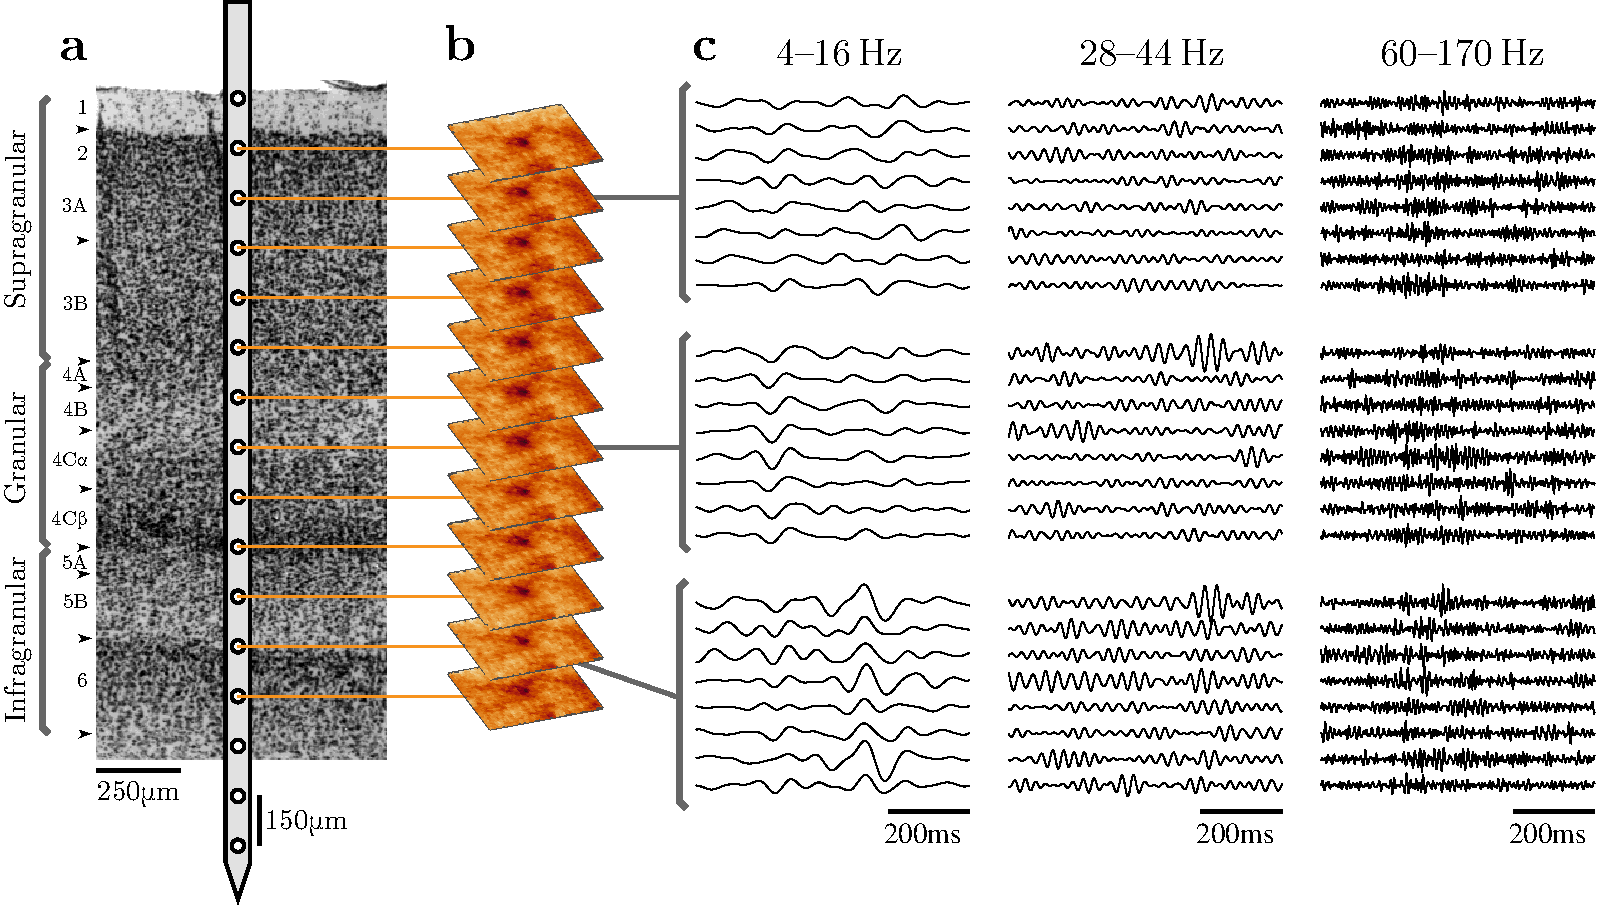
\includegraphics[width=\linewidth]{paperfigs/fig1.pdf}
}
%
\caption{
\captionemph{Overview of data collection and example data.}
\protect\subref{fig:lam_1a}:~Illustration of experimental recording setup, showing approximate locations of electrode contacts in relation to a Nissl stained section of macaque \ac{V1} cortex.
Boundaries between cortical laminae are indicated with arrowheads.
% (Electrode width not to scale.)
Stain reprinted from \citet{Tyler1998}, with permission (Copyright \copyright{} 1998 Wiley-Liss, Inc).
% Permission is granted subject to an appropriate acknowledgement given to the author, title of the material/book/journal and the publisher. You shall also duplicate the copyright notice that appears in the Wiley publication in your use of the Wiley Material.
\protect\subref{fig:lam_1b}:~Receptive field locations were consistent across the cortical depth.
Location of receptive field for each cortical recording site was identified by reverse correlating the \ac{MUA} with the luminance changes of each pixel in the movie (session \sesname{E07nm1}).
\protect\subref{fig:lam_1c}:~Example \ac{CSD} traces from simultaneous recordings at three cortical depths for eight repetitions of a movie fragment (session \sesname{H05nm7}).
The data is split into three temporal frequency bands (\SIrange{4}{16}{Hz}, \SIrange{28}{44}{Hz}, and \SIrange{60}{170}{Hz}).
}%
\label{fig:lam_1}
%
\end{figure}


\subsection{Distribution of information across depth and frequency}

We considered how neural activity in different frequency bands changed in response to the movie.
To visually convey how information is encoded into different frequency bands (\autoref{fig:lam_1c}), we filtered the \ac{CSD} at three cortical depths in three spectral bands during eight presentations of a portion of the movie clip.
Within this small sample of the overall dataset, one can observe that large, low-frequency deflections in the activity are consistent across trials within \ac{G} and \ac{IG} depths, and the envelope-amplitude of activity in the \SIrange{60}{170}{Hz} band is also consistent across trials, most clearly for the \ac{SG} compartment.
Activity in the \SIrange{28}{44}{Hz} range was more variable across trials, and did not seem to be stimulus modulated.


\begin{figure}[htbp]%
    \centering
    \hspace*{\fill}
    \subfloat[][\acs{LFP} power.\label{fig:lam_power_lfp}]{%
        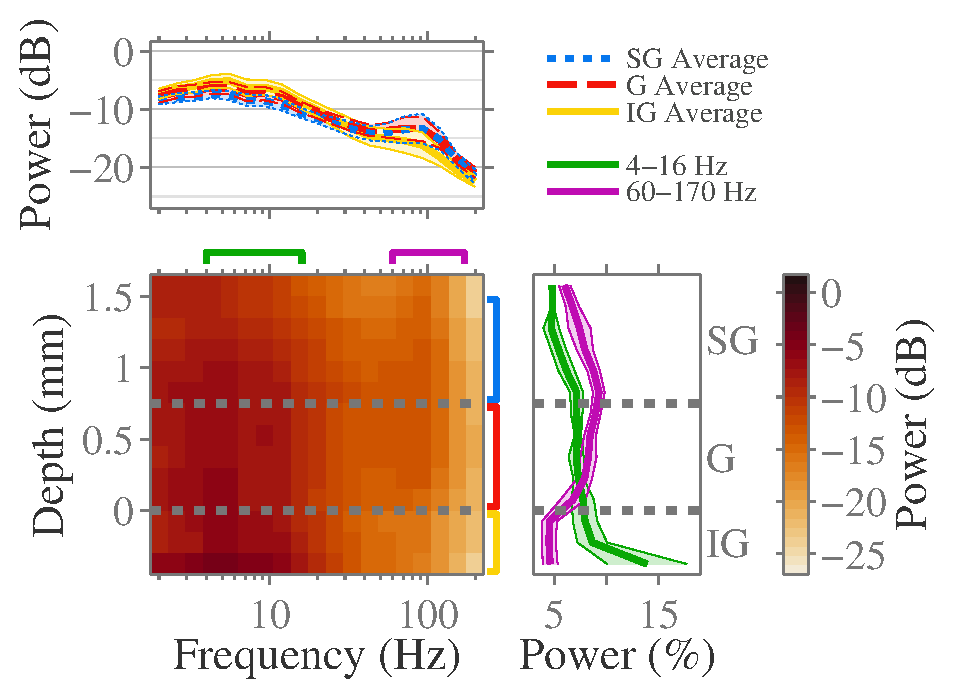
\includegraphics[scale=.325]{%
figs/info/fig3set-logRsp-Cln-power-straightnangeomean-compzonescb-legend.eps}}
    \hspace*{\fill}\hspace{.2cm}\hspace*{\fill}
    \subfloat[][\acs{CSD} power.\label{fig:lam_power_csd}]{%
        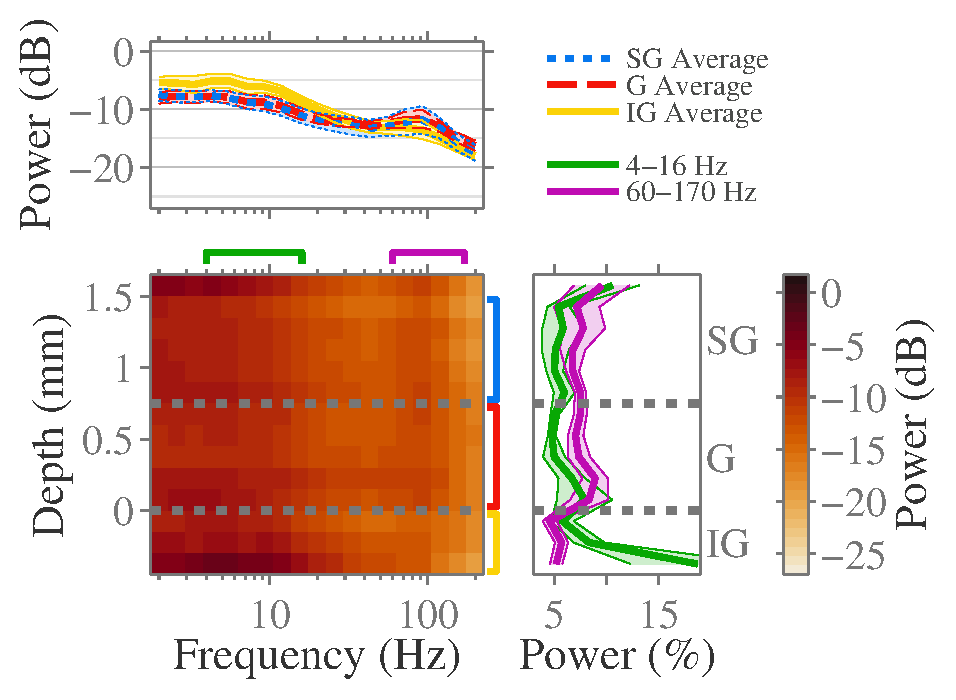
\includegraphics[scale=.325]{%
figs/info/fig3set-logRsp-Csd-power-straightnangeomean-compzonescb-legend.eps}}
    \hspace*{\fill}
    \\
    \hspace*{\fill}
    \subfloat[][\acs{LFP} information.\label{fig:lam_info_lfp}]{%
        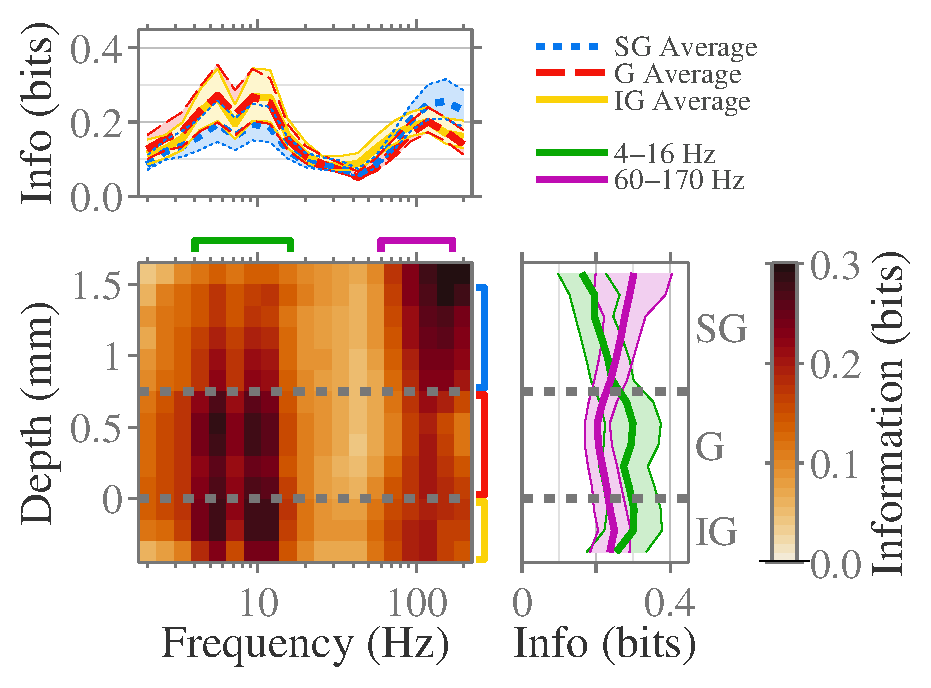
\includegraphics[scale=.325]{%
figs/info/fig3set-info-Cln-power-straightnanmean-compzonescb-legend.eps}}
    \hspace*{\fill}\hspace{.2cm}\hspace*{\fill}
    \subfloat[][\acs{CSD} information.\label{fig:lam_info_csd}]{%
        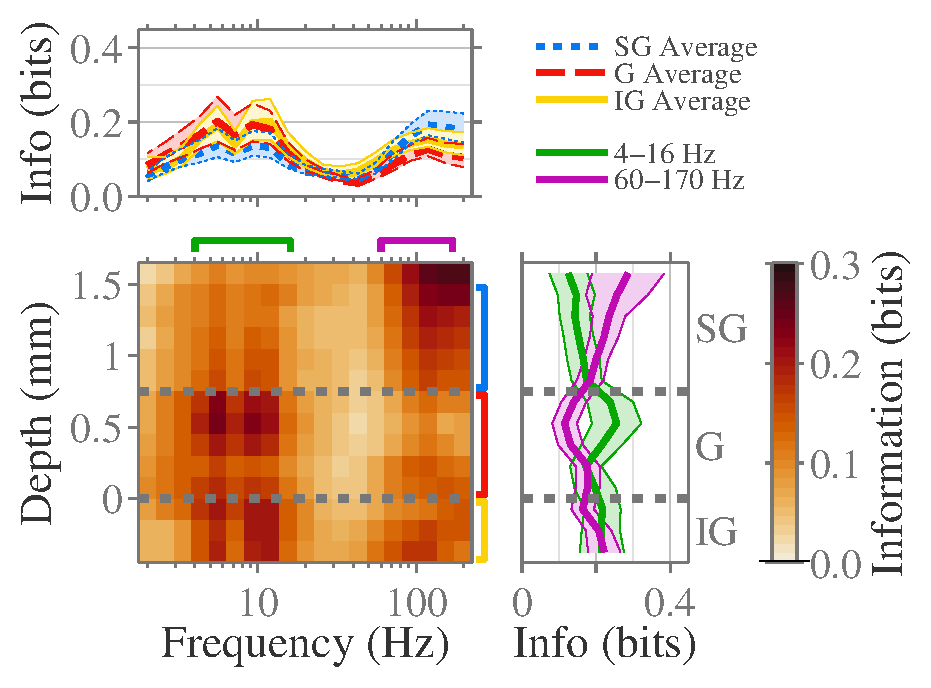
\includegraphics[scale=.325]{%
figs/info/fig3set-info-Csd-power-straightnanmean-compzonescb-legend.eps}}
    \hspace*{\fill}
    \caption{
\captionemph{Distribution of visual stimulus information across both cortical depth and frequency.}
\protect\subref{fig:lam_power_lfp}:~Distribution of \ac{LFP} power during stimulus presentation.
Plot shows the geometric mean power over \num{6} sessions.
Above, mean power within \ac{SG}, \ac{G} and \ac{IG} compartments.
Right, laminar distribution of \ac{LFP} power in \SIrange{4}{16}{Hz} and \SIrange{60}{170}{Hz} frequency bands.
\protect\subref{fig:lam_power_csd}:~Same as \protect\subref{fig:lam_power_lfp}, but distribution of \ac{CSD} power instead of \ac{LFP} power.
\protect\subref{fig:lam_info_lfp}:~Distribution of information about the stimulus contained in \ac{LFP} power.
Plot shows the mean information over \num{6} sessions.
Above, mean information within \ac{SG}, \ac{G} and \ac{IG} compartments.
Right, cortical distribution of information in the power in \SIrange{4}{16}{Hz} and \SIrange{60}{170}{Hz} frequency bands.
\protect\subref{fig:lam_info_csd}:~Same as \protect\subref{fig:lam_info_lfp}, but for information in \ac{CSD} power instead of \ac{LFP} power.
Note that the information, \protect\subref{fig:lam_info_lfp} and \protect\subref{fig:lam_info_csd}, is distributed very differently from the \ac{LFP} and \ac{CSD} power, \protect\subref{fig:lam_power_lfp} and \protect\subref{fig:lam_power_csd}.
Each datapoint in \protect\subref{fig:lam_info_lfp} and \protect\subref{fig:lam_info_csd} was tested for statistical significance using bootstrapping, and each datapoint was found to be significant.
    \label{fig:lam_info}
}
\end{figure}

We quantified these observations by computing how much information the spectral power of the \ac{LFP} and \ac{CSD} contain about the identity of which movie frame is currently on screen (see \autoref{sec:lam_info_method}).
Despite the fact that the power is distributed evenly across depth and decays smoothly as frequency increases (Figures \ref{fig:lam_power_lfp} and \ref{fig:lam_power_csd}), we found that information in the spectral power was localised around particular depths and frequencies (Figures \ref{fig:lam_info_lfp} and \ref{fig:lam_info_csd}).

For both \ac{LFP} and \ac{CSD}, information about the movie is highest in the \SIrange{4}{16}{Hz} range at the top of the granular (\acs{G}) compartment (layer 4A/B), and \SI{>60}{Hz} near the top of the \ac{SG} compartment (layer 2).
Additionally, there are secondary local maxima in \ac{IG} for both the \SIrange{4}{16}{Hz} and \SIrange{60}{150}{Hz} ranges.
These results are consistent across all individual recording sessions (\autoref{fig:lam_info_sessions}).
Since \ac{LFP} and \ac{CSD} have the same distribution of information, but the \ac{CSD} has better spatial localisation than the \ac{LFP} \citep{Einevoll2013,Kajikawa2011}, we will restrict ourselves to only studying the \ac{CSD} for the remainder of the chapter.

\begin{figure}
% \centering 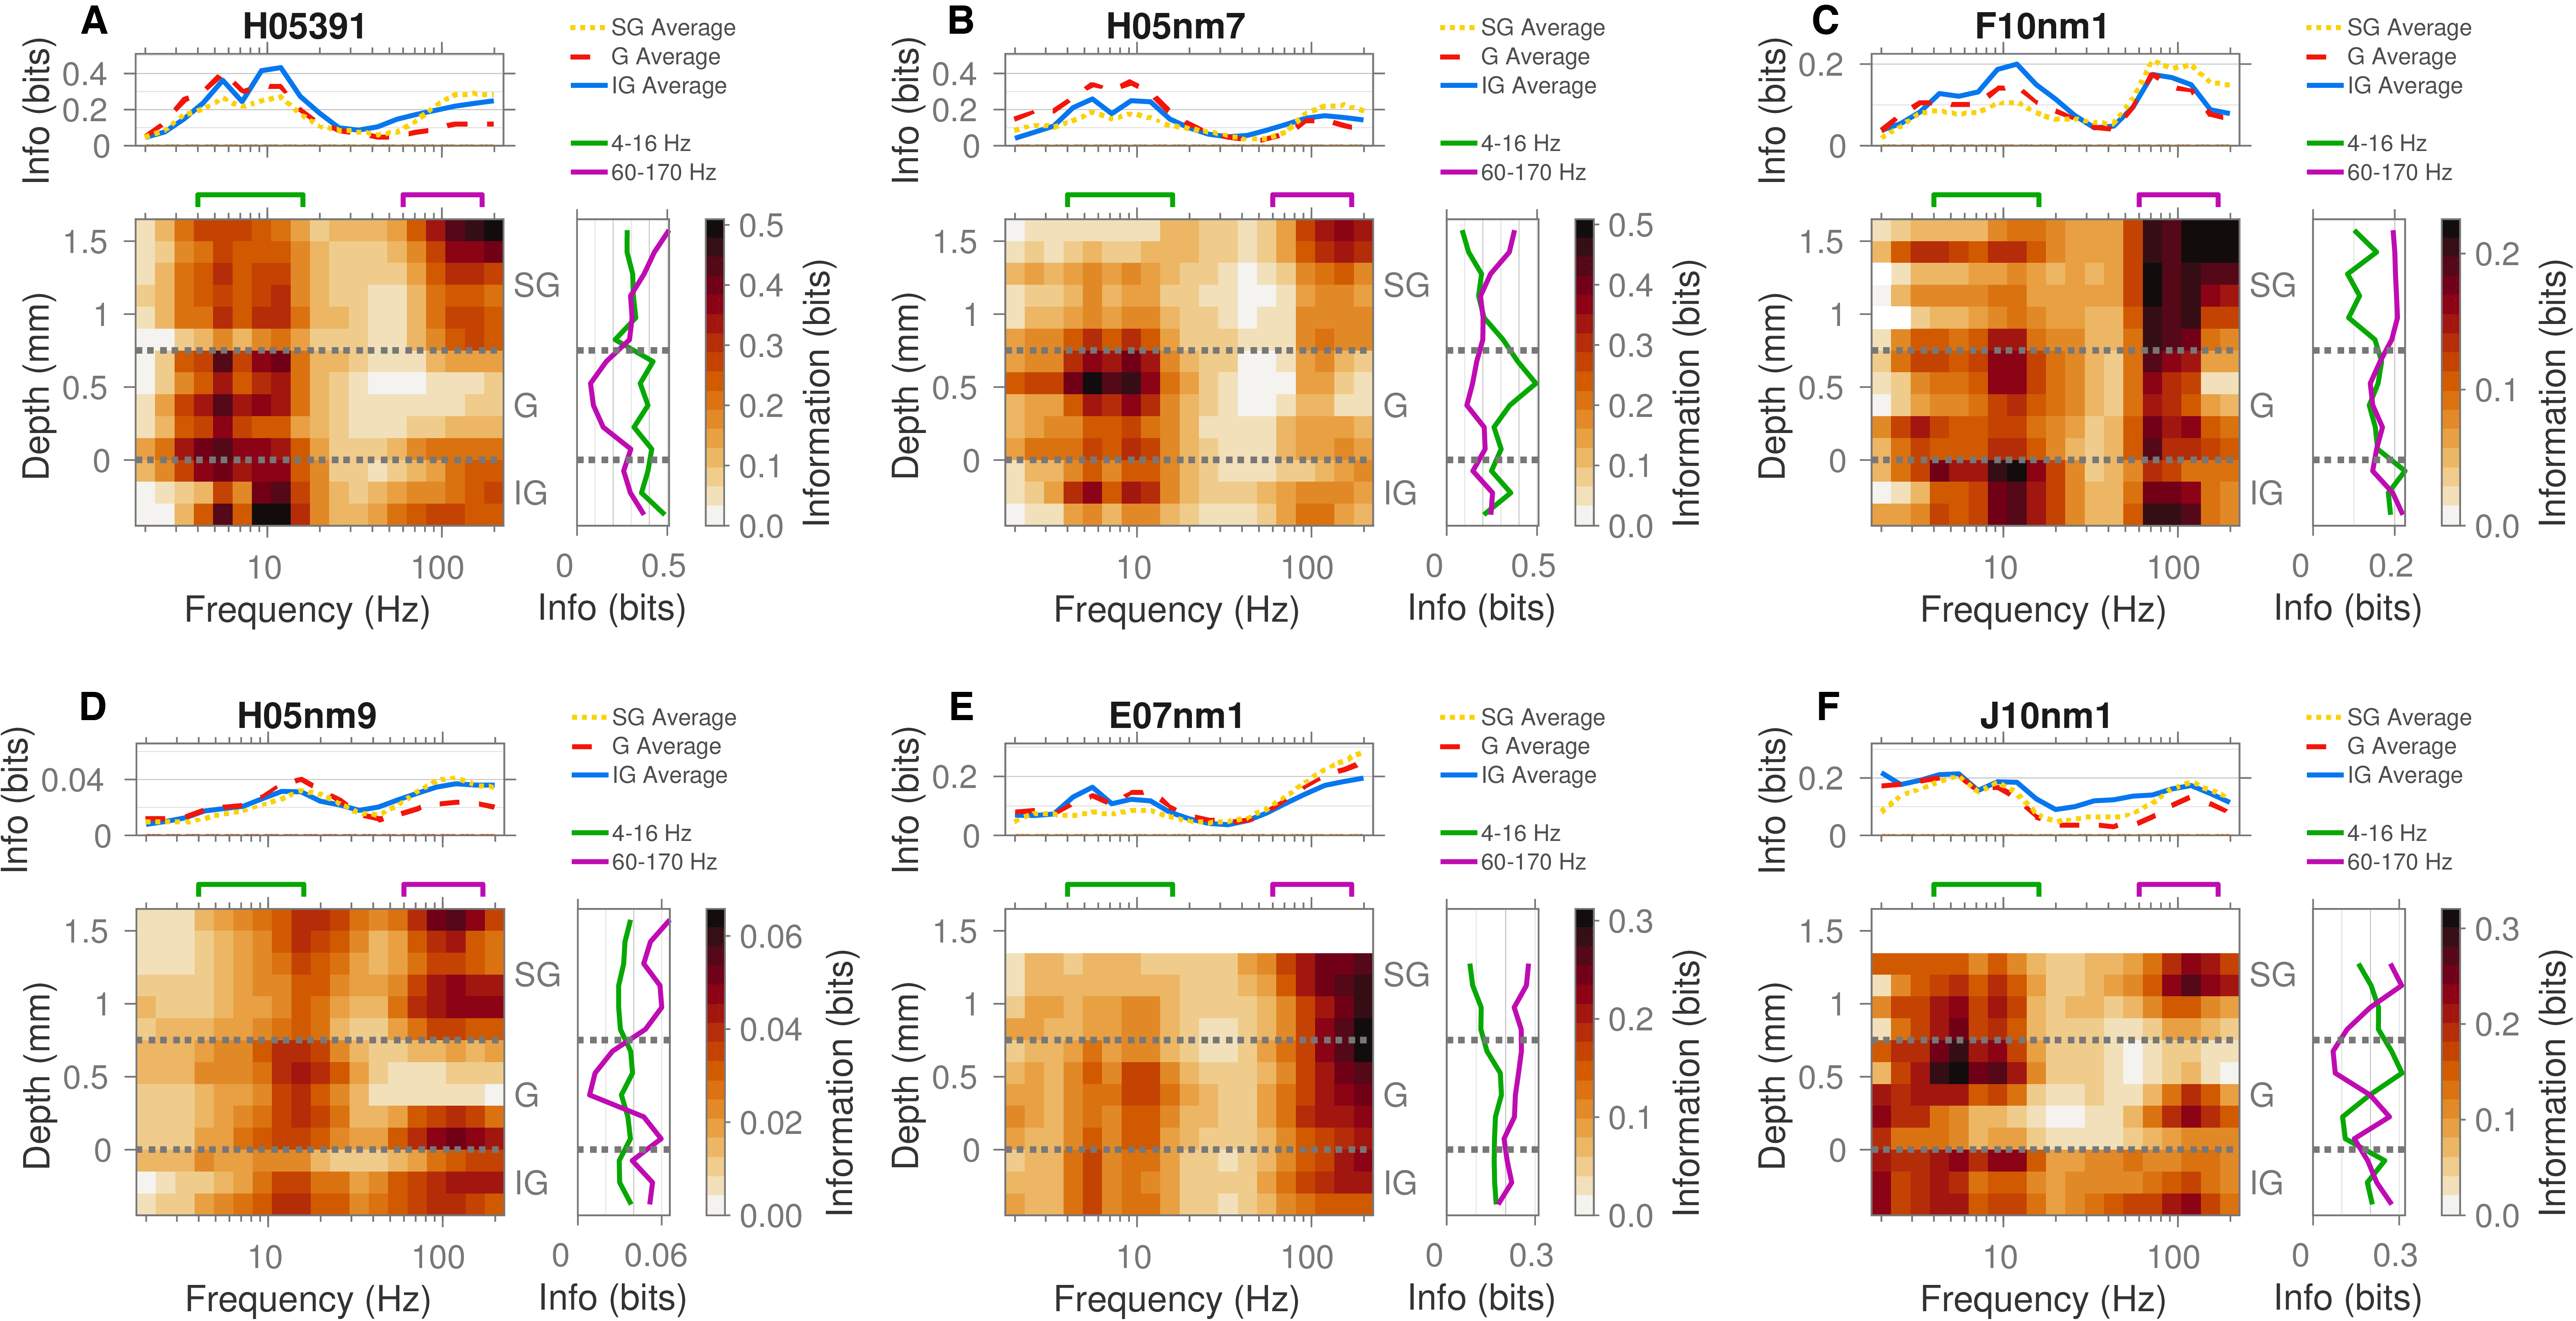
\includegraphics[width=\columnwidth]{paperfigs/figS2}
    \centering
    \hspace*{\fill}
    \subfloat[][\sesname{H05391} \acs{CSD} information.]{%
        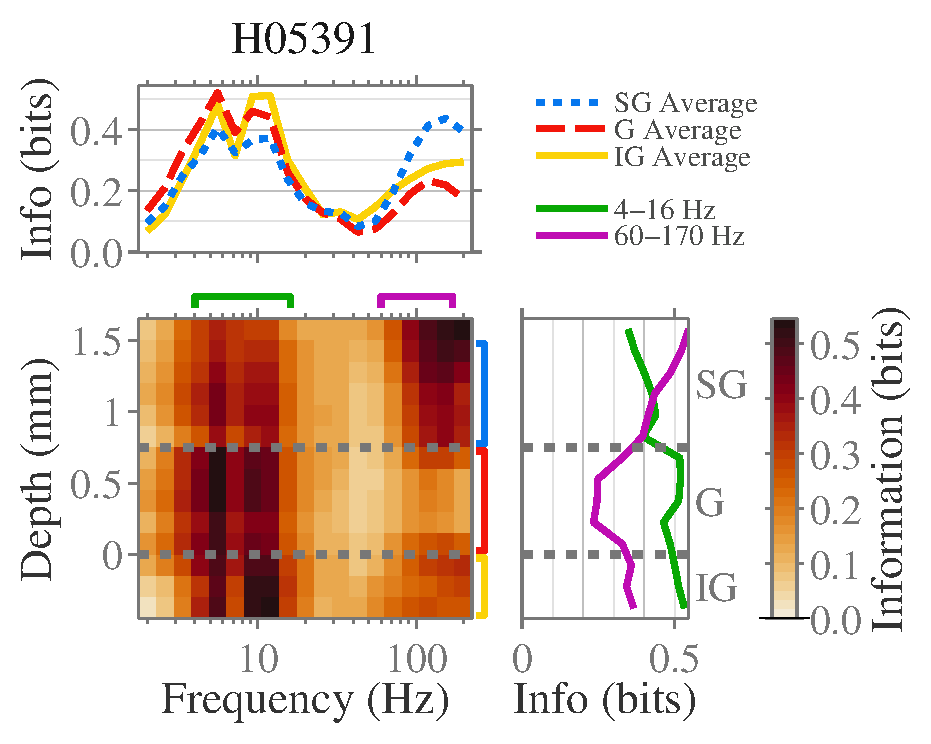
\includegraphics[scale=.325]{%
figs/info-sessions/fig3set-info-Cln-power-H05391-compzonescb-legend.eps}}
    \hspace*{\fill}\hspace{.2cm}\hspace*{\fill}
    \subfloat[][\sesname{H05nm9} \acs{CSD} information.]{%
        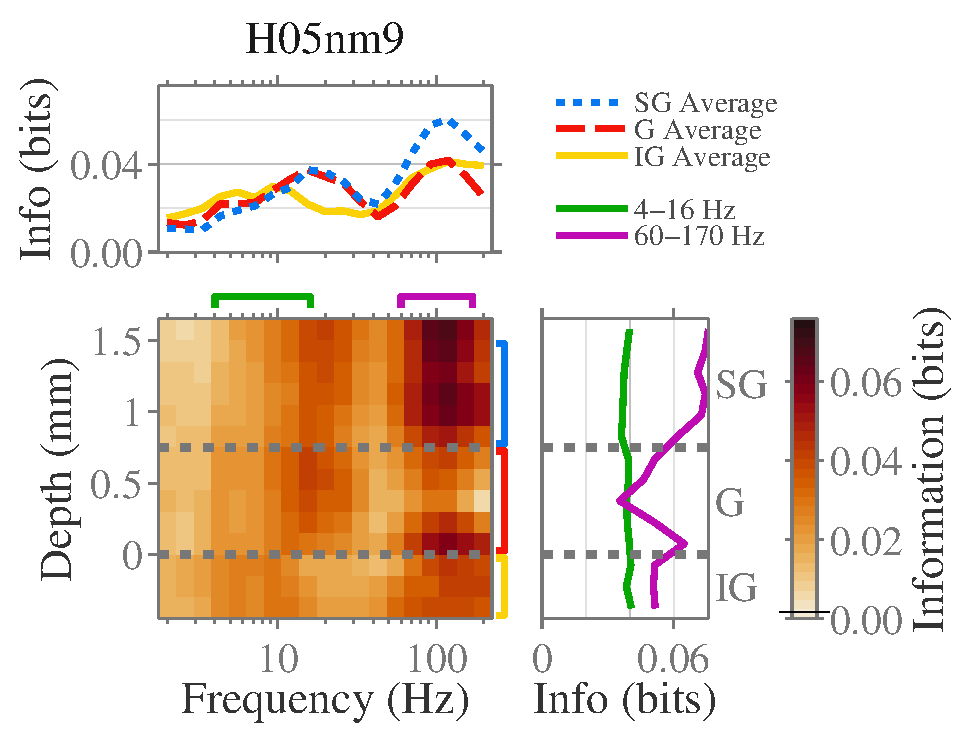
\includegraphics[scale=.325]{%
figs/info-sessions/fig3set-info-Cln-power-H05nm9-compzonescb-legend.eps}}
    \hspace*{\fill}
    \\
    \hspace*{\fill}
    \subfloat[][\sesname{H05nm7} \acs{CSD} information.]{%
        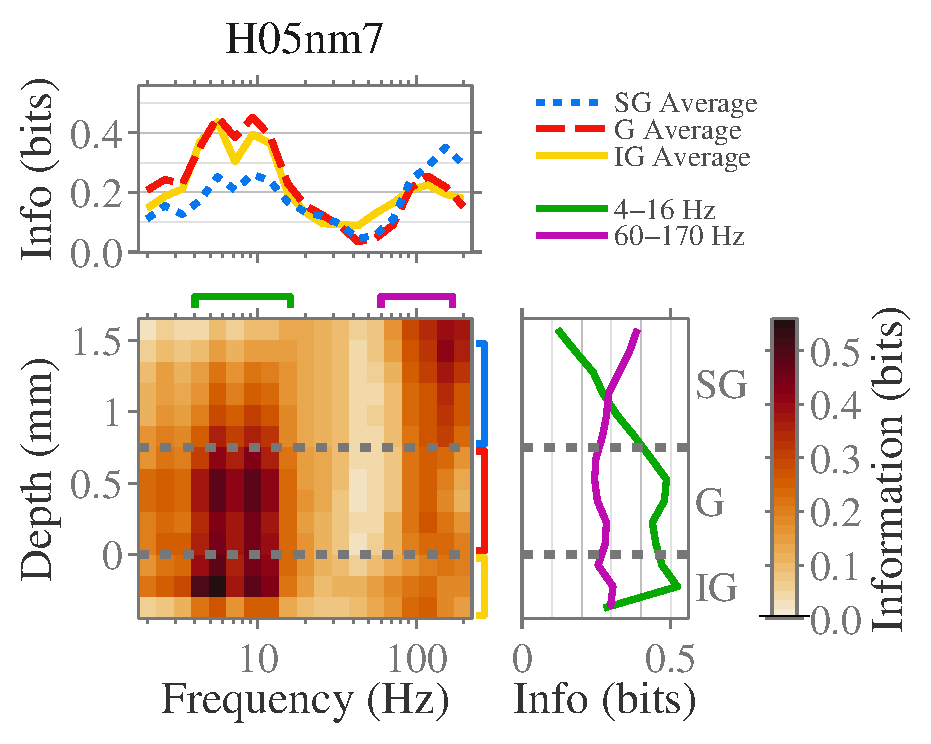
\includegraphics[scale=.325]{%
figs/info-sessions/fig3set-info-Cln-power-H05nm7-compzonescb-legend.eps}}
    \hspace*{\fill}\hspace{.2cm}\hspace*{\fill}
    \subfloat[][\sesname{E07nm1} \acs{CSD} information.]{%
        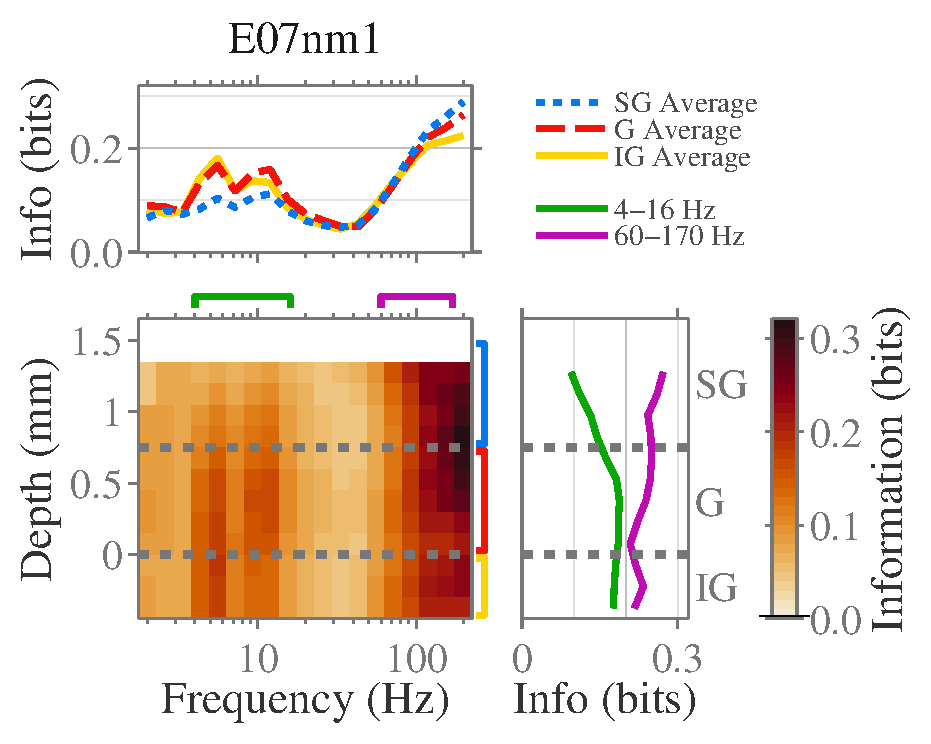
\includegraphics[scale=.325]{%
figs/info-sessions/fig3set-info-Cln-power-E07nm1-compzonescb-legend.eps}}
    \hspace*{\fill}
    \\
    \hspace*{\fill}
    \subfloat[][\sesname{F10nm1} \acs{CSD} information.]{%
        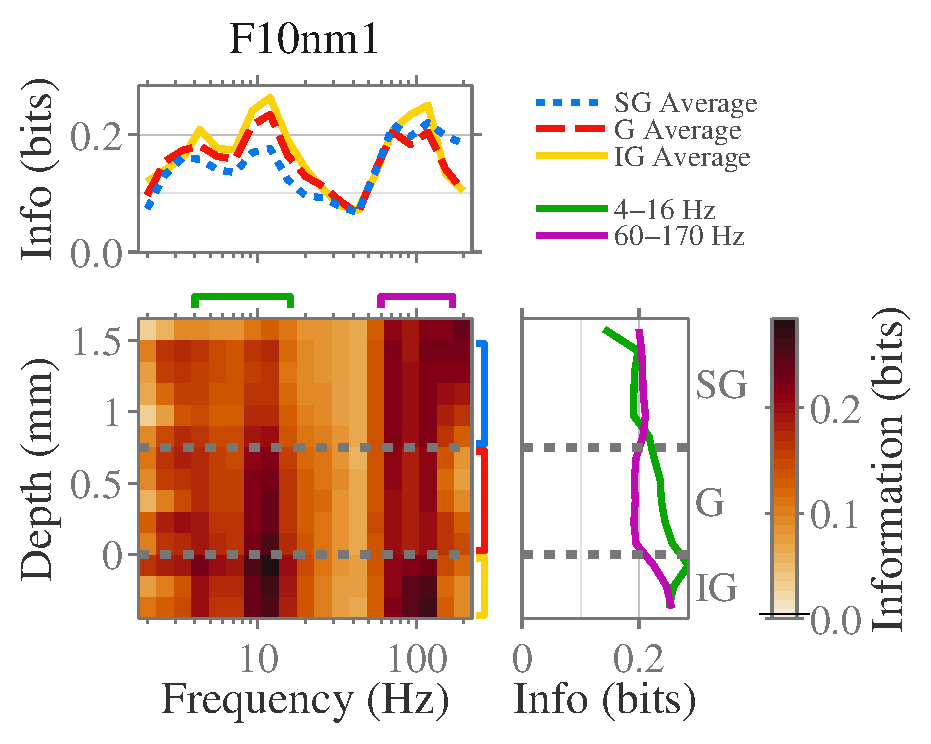
\includegraphics[scale=.325]{%
figs/info-sessions/fig3set-info-Cln-power-F10nm1-compzonescb-legend.eps}}
    \hspace*{\fill}\hspace{.2cm}\hspace*{\fill}
    \subfloat[][\sesname{J10nm1} \acs{CSD} information.]{%
        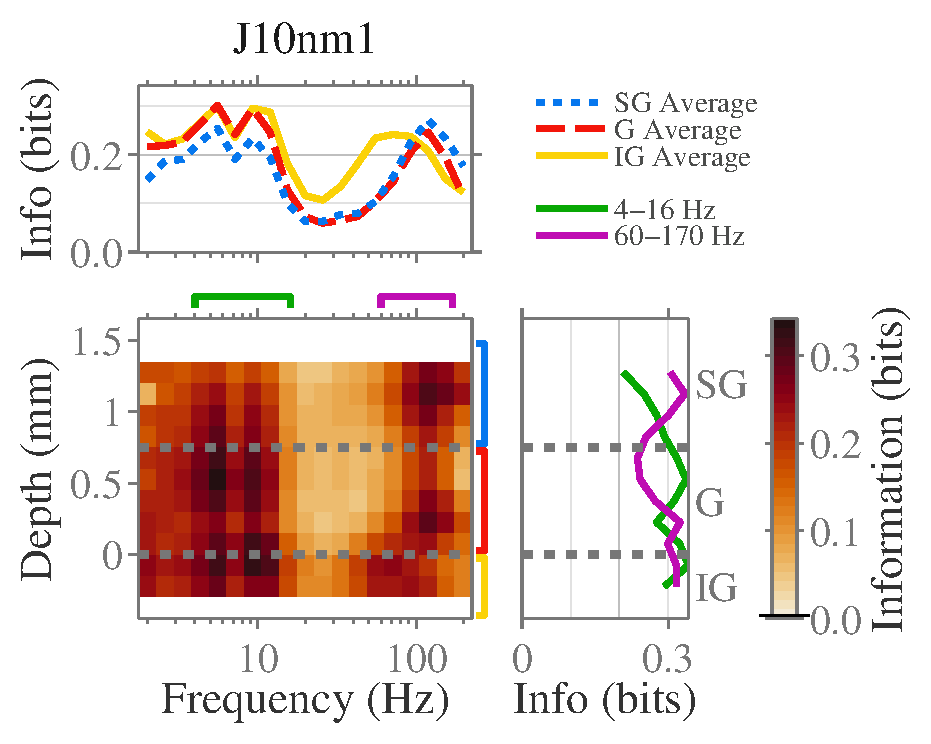
\includegraphics[scale=.325]{%
figs/info-sessions/fig3set-info-Cln-power-J10nm1-compzonescb-legend.eps}}
    \hspace*{\fill}
%
\caption{
\captionemph{Distribution of information about the movie across both cortical depth and frequency for individual sessions}
Same as \autoref{fig:lam_info_csd}, but shown for each recording session individually.
}
\label{fig:lam_info_sessions}
%
\end{figure}

These results suggest that within a single neocortical column there are two frequency bands which act as stimulus-encoding channels, which are approximately the \SIrange{4}{16}{Hz} and \SIrange{60}{170}{Hz} frequency ranges.


\subsection{Information redundancy between frequencies}
\label{sec:lam_redundancy}

These results raise the question whether the two frequency ranges (\SIrange{4}{16}{Hz} and \SIrange{60}{170}{Hz}) encode the same or different information about the stimulus, and whether the same information is encoded within a given frequency band across the entire cortical depth. 
To answer this, we computed the redundancy between pairs of frequency bands of the information about the stimulus which they encode (see \autoref{sec:lam_redundancy_method}).
Computing information redundancy allows us to quantify how similar the information about the stimulus is for a given pair of frequency bands and depths --- high redundancy shows the information about the stimulus is mostly the same in the two bands, low redundancy means the two bands contain independent information about the stimulus.

\begin{figure}[htbp]
\centering
\begin{tabular}{ll}
\subfloat[][Redundancy between frequencies.\label{fig:lam_cxfrq_red}]{%
    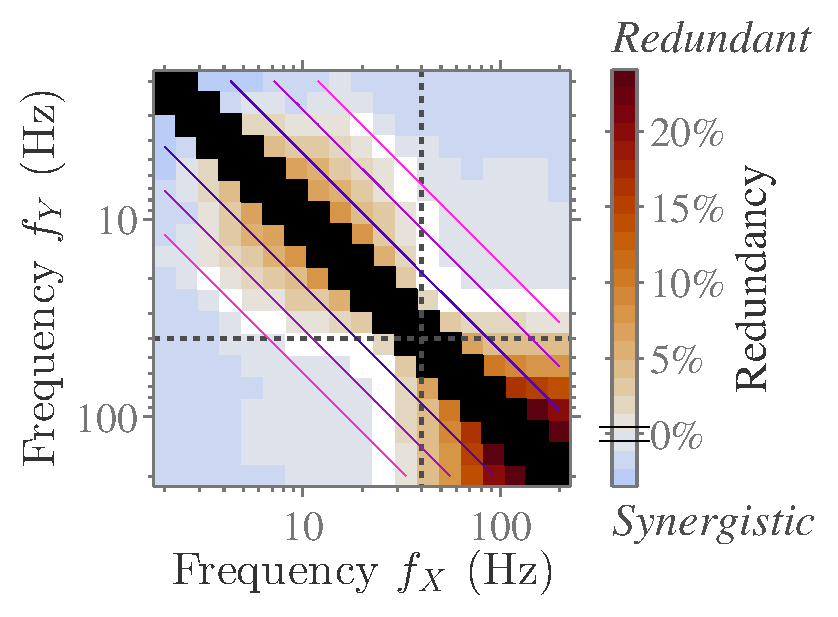
\includegraphics[scale=.34]{figs/redundancy/cxsfrq-pcred_power-power_avg-log.eps}}
&
\subfloat[][Information gain between frequencies.\label{fig:lam_cxfrq_gain}]{%
    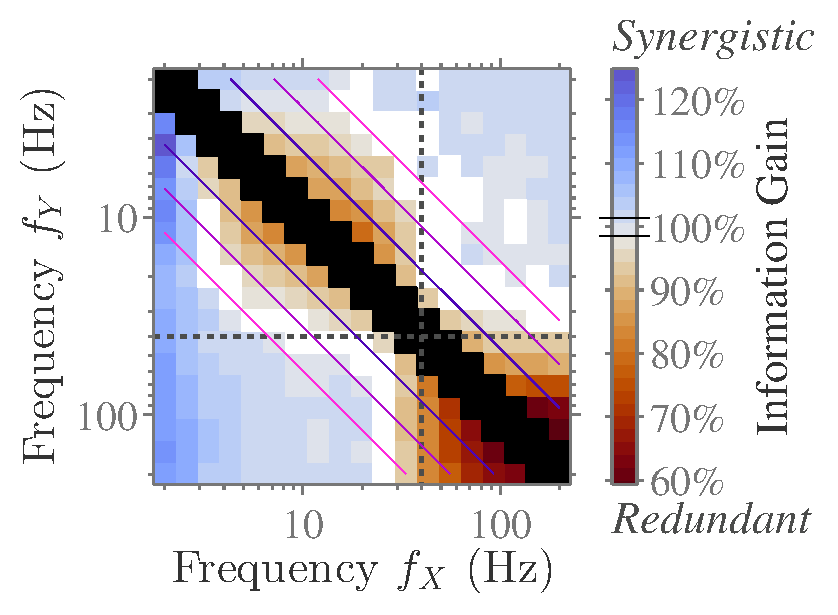
\includegraphics[scale=.34]{%
figs/redundancy/cxsfrq-pcgain-i2d2_power-power_avg-log.eps}}
% (I12 - I1) / I2, 1 on y-axis, 2 on x-axis
\\
\subfloat[][Redundancy cross-section.\label{fig:lam_cxfrq_red_diag}]{%
    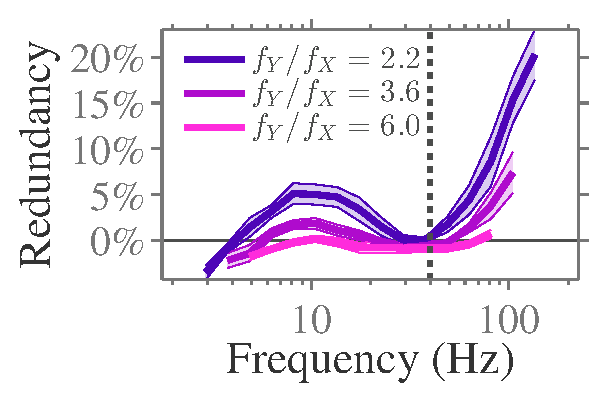
\includegraphics[scale=.34]{%
figs/redundancy/cxsfrq-pcred_power-power_avg-log_diagonal.eps}}
&
\subfloat[][Information gain cross-section.\label{fig:lam_cxfrq_gain_diag}]{%
    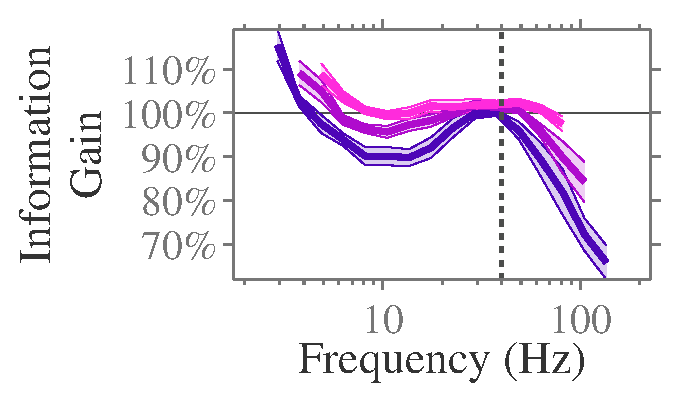
\includegraphics[scale=.34]{%
figs/redundancy/cxsfrq-pcgain-i2d2_power-power_avg-log_diagonal_noleg.eps}}
\end{tabular}
%
\caption{
\captionemph{Information redundancy between \ac{CSD} frequency components.}
\protect\subref{fig:lam_cxfrq_red}:~Redundancy (as defined in \autoref{eq:redundancy}) between pairs of frequencies, averaged over all cortical recording depths, then averaged over \num{6} sessions.
Each datapoint was tested for statistical significance using bootstrapping, and non-significant values are shown in white (the median threshold for statistical significance is shown as a line across the colour bar).
The leading diagonal, which is trivially redundant, and second diagonal, which is highly redundant due to the \SI{50}{\percent} overlap between neighbouring frequency bands, are removed (black).
\protect\subref{fig:lam_cxfrq_gain}:~Same as \protect\subref{fig:lam_cxfrq_red}, but for the asymmetric information gain $\operatorname{InfoGain}\left(Y\to\left\{X,Y\right\};S\right)$ (defined in \autoref{eq:infogain}).
\protect\subref{fig:lam_cxfrq_red_diag}:~Redundancy between pairs of bands with a fixed ratio between their frequencies, plotted against the geometric mean of their band centres.
The shaded region indicates the standard error on the mean over \num{6} sessions.
\protect\subref{fig:lam_cxfrq_gain_diag}:~Same as \protect\subref{fig:lam_cxfrq_red_diag}, but for the information gain.
We averaged over both $Y \to \{X,Y\}$ and $X \to \{X,Y\}$ for each pair of frequencies when tracing the information gain between pairs of channels with constant frequency ratio.
}%
\label{fig:lam_cxfrq_info}
%
\end{figure}

As shown in \autoref{fig:lam_cxfrq_info}, we found there are two frequency domains within which information is redundant: \SIrange{4}{40}{Hz} and \SI{>40}{Hz}.
Furthermore, the information contained in neural frequencies \SI{<40}{Hz} is different to the information contained in frequencies \SI{>40}{Hz}, since we measured these to be independent (redundancy \SI{\le0}{\percent}, information gain \SI{\ge100}{\percent}.
Additionally, we note that the same \SI{<40}{Hz} and \SI{>40}{Hz} division is observed for the signal correlation (\autoref{fig:lam_cxfrq_cor}), and our results corroborate earlier findings \citep{Belitski2008}.
Taken together, our results thus show that the two bands (\SIrange{4}{16}{Hz} and \SIrange{60}{170}{Hz}) contain the most information about the stimulus and encode different information about the stimulus.

\begin{figure}[htbp]
\centering
\begin{tabular}{ll}
\subfloat[][Signal correlation between frequencies.\label{fig:lam_cxfrq_sigcor}]{%
    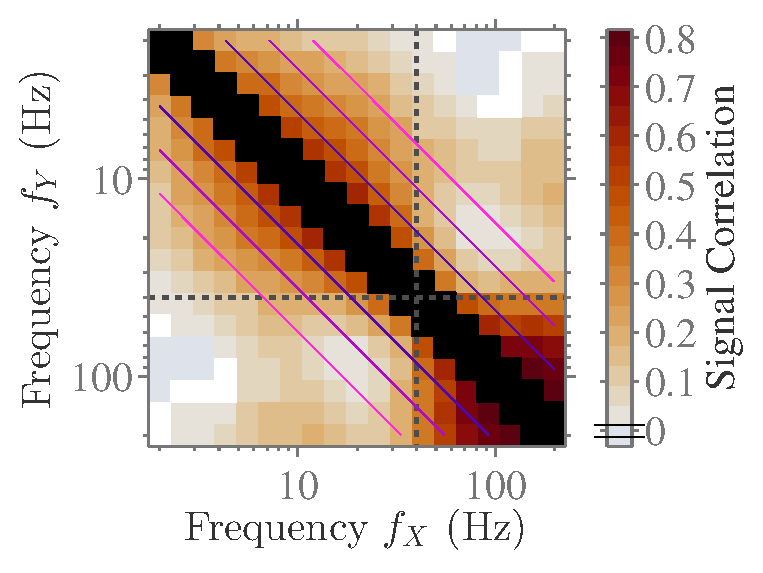
\includegraphics[scale=.34]{%
figs/noisesigcor/cxsfrq-signal-power-power-avg-log.eps}}
&
\subfloat[][Noise correlation between frequencies.\label{fig:lam_cxfrq_noisecor}]{%
    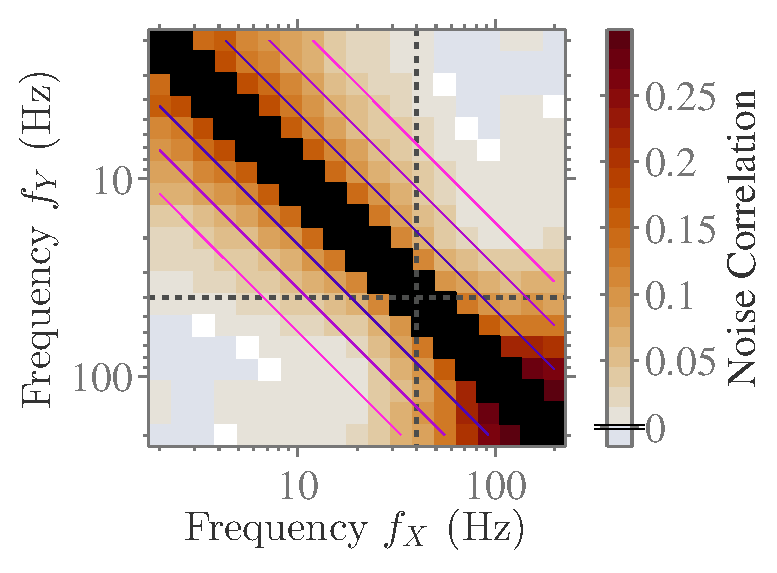
\includegraphics[scale=.34]{%
figs/noisesigcor/cxsfrq-noise-power-power-avg-log.eps}}
\\
\subfloat[][Signal correlation cross-section.\label{fig:lam_cxfrq_sigcor_diag}]{%
    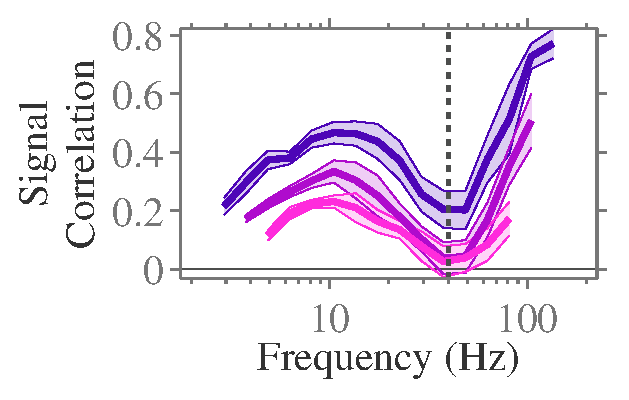
\includegraphics[scale=.34]{%
figs/noisesigcor/cxsfrq-signal-power-power-avg-log_diagonal_noleg.eps}}
&
\subfloat[][Noise correlation cross-section.\label{fig:lam_cxfrq_noisecor_diag}]{%
    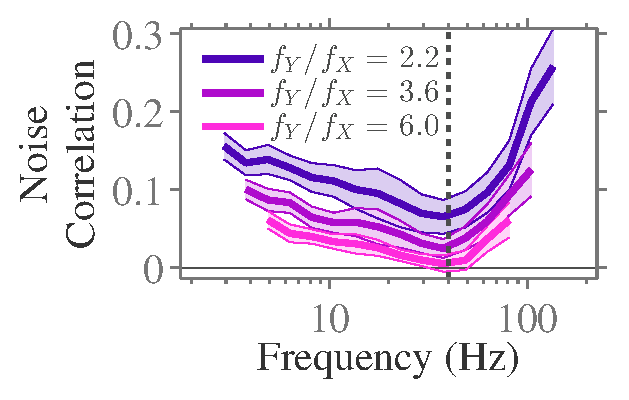
\includegraphics[scale=.34]{%
figs/noisesigcor/cxsfrq-noise-power-power-avg-log_diagonal.eps}}
\end{tabular}
%
\caption{
\captionemph{Correlation between \ac{CSD} frequency bands.}
\protect\subref{fig:lam_cxfrq_sigcor}:~Signal correlation between the power in pairs of frequencies, median across \numrange{12}{14} cortical recording sites, mean over \num{6} sessions.
The leading diagonal, which is trivially perfectly correlated, and second diagonal, which is highly correlated due to the \SI{50}{\percent} overlap between neighbouring frequency bands, are removed (black).
\protect\subref{fig:lam_cxfrq_noisecor}:~Noise correlation between the power in pairs of frequencies, median across \numrange{12}{14} cortical recording sites, mean over \num{6} sessions.
\protect\subref{fig:lam_cxfrq_sigcor_diag}:~As per \autoref{fig:lam_cxfrq_red_diag}, the signal correlation between pair of frequencies with a fixed ratio between their frequencies, plotted against the geometric mean of their band centres.
\protect\subref{fig:lam_cxfrq_noisecor_diag}:~Same as \protect\subref{fig:lam_cxfrq_sigcor_diag}, but for noise correlation.
}%
\label{fig:lam_cxfrq_cor}
%
\end{figure}


\subsection{Information redundancy across depth}

Next, we investigated whether the information contained in these frequency bands was the same across the cortical depths.
To this end, we computed the redundancy of the information about the stimulus contained in oscillations at different cortical depths, both within the same band at each depth, and between different bands (\autoref{fig:lam_cxchn_info}; see \autoref{sec:lam_redundancy_method}).

\begin{figure}[htbp]
    \centering
    \hspace*{\fill}
    \subfloat[][Redundancy.\label{fig:lam_cxchn_red}]{%
        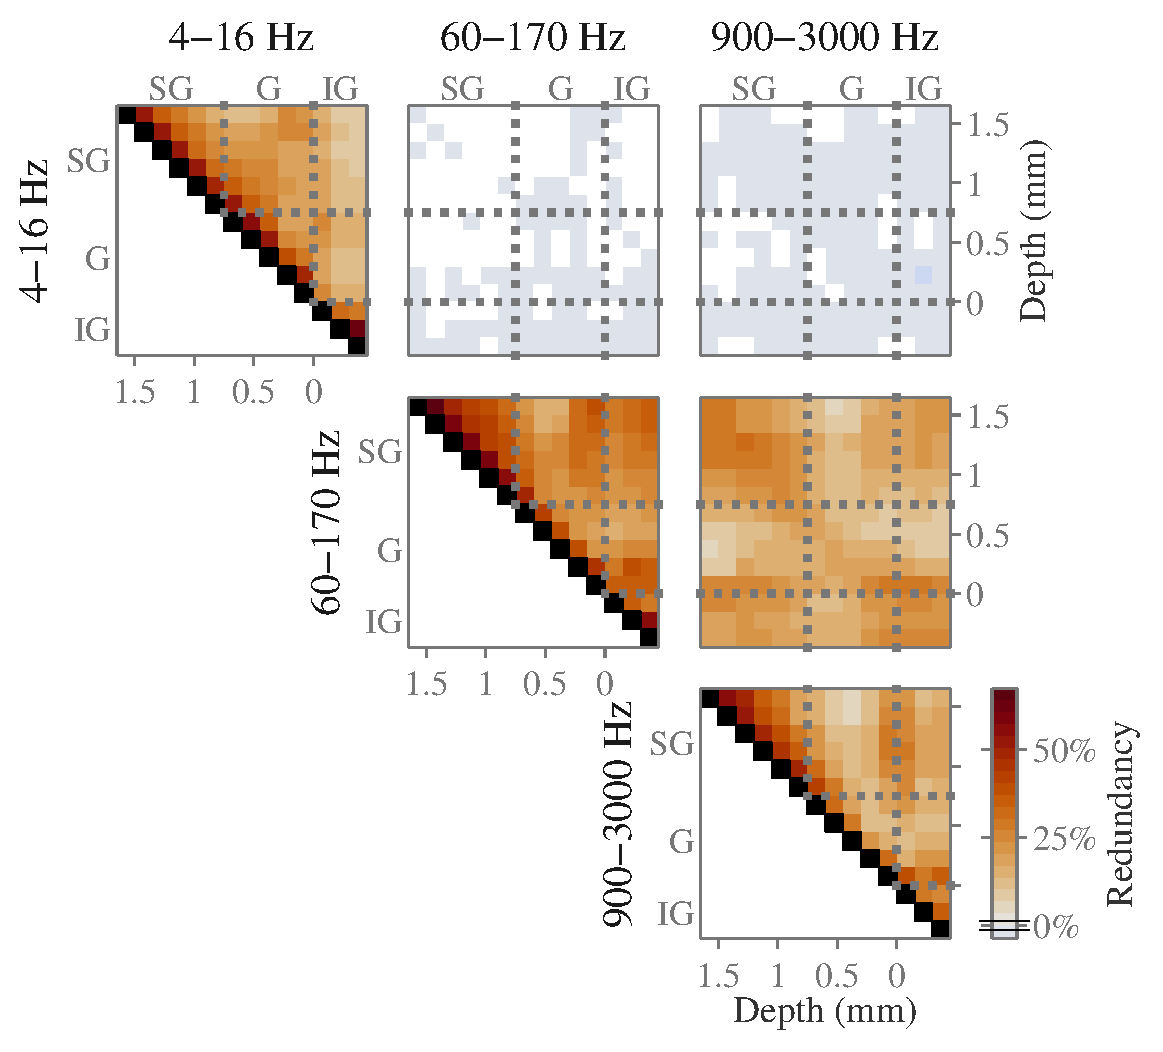
\includegraphics[scale=.34]{%
figs/redundancy/bndflt3-3-pcred-none-avg-lag=0s_paper.eps}}
    \hspace*{\fill}
    \\
    \hspace*{\fill}
    \subfloat[][Information gain.\label{fig:lam_cxchn_gain}]{%
        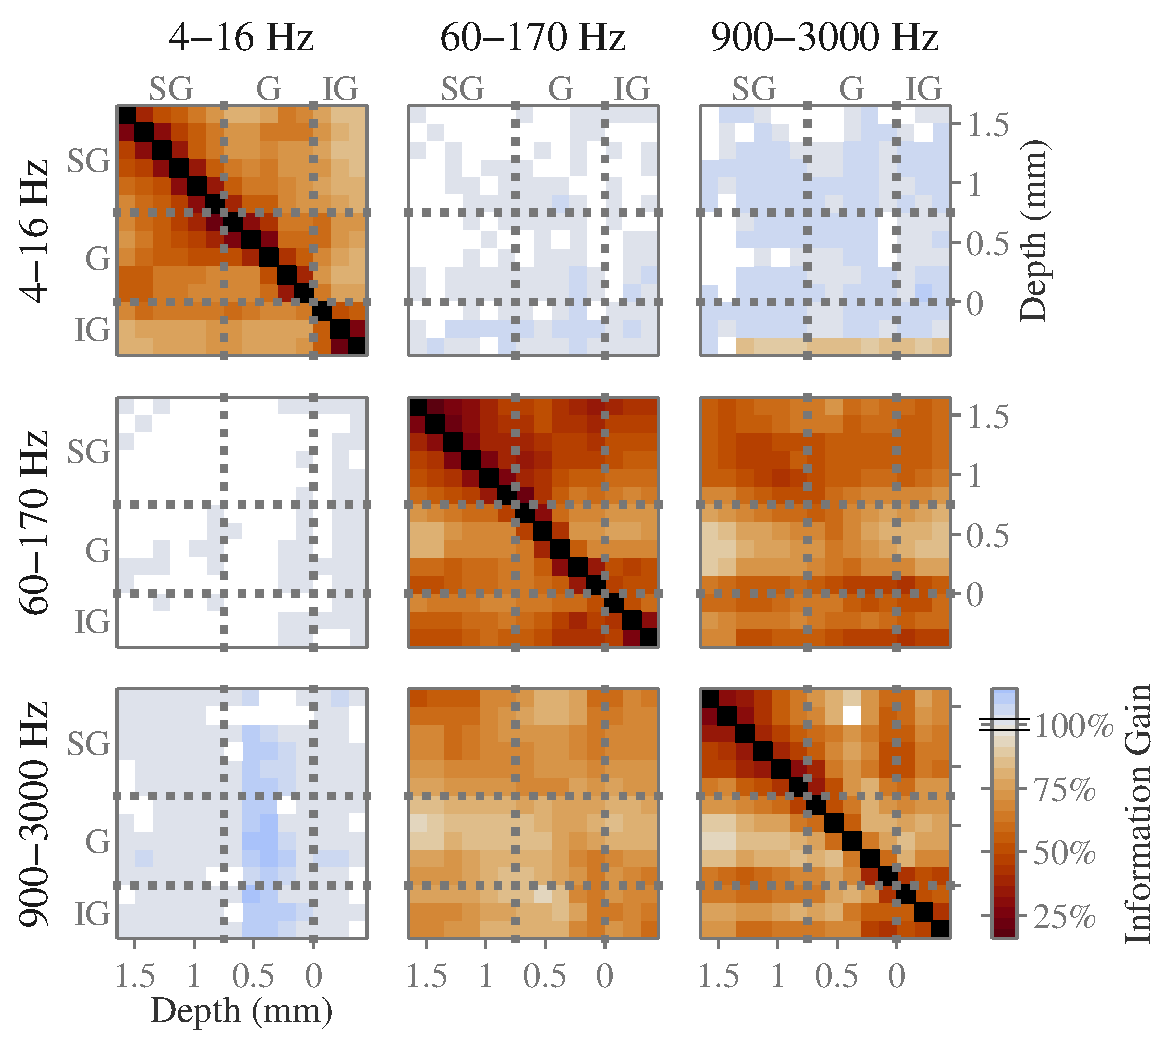
\includegraphics[scale=.34]{%
figs/redundancy/bndflt3-3-pcgain-i2d2-none-avg-lag=0s_paper.eps}}
    \hspace*{\fill}
%
\caption{
\captionemph{Redundancy of information contained in pairs of cortical laminae, for isolated \ac{CSD} frequency bands and \ac{MUA}.}
We show both the redundancy, \protect\subref{fig:lam_cxchn_red}, and the information gain, $\operatorname{InfoGain}\left(Y\to\left\{X,Y\right\};S\right)$, \protect\subref{fig:lam_cxchn_gain}.
Since redundancy, as we define in \autoref{eq:redundancy}, is symmetric, the lower triangle (removed) is a mirror image of the upper triangle.
Information gain is an asymmetric measure, and we show the gain from knowing the $y$-axis datapoint to knowing both $x$ and $y$ datapoints.
Non-significant datapoints are shown in white, with the median upper and lower thresholds for significance indicated by the black lines across each colour bar.
}%
\label{fig:lam_cxchn_info}
%
\end{figure}

Within the \SIrange{4}{16}{Hz} frequency range, there is redundancy across the entire cortical depth, but there are two distinct cortical compartments (above and below the \ac{CSD} reversal, marked as \SI{0}{mm} depth) within which there is increased redundancy.
These findings are in agreement with \citet{Maier2010}, who found a transition corresponding to the \ac{G}/\ac{IG} boundary which isolated two cortical compartments with high coherence for \ac{LFP} oscillations \SI{<100}{Hz}.
We also find that gamma oscillations (\SIrange{60}{170}{Hz}) have substantial redundancy across the cortical depth.

We investigated the redundancy between cortical oscillations and spiking activity by extracting the power of the \SIrange{900}{3000}{Hz} frequency range which indicates the aggregate \acf{MUA}.
The information in the \ac{MUA} is redundant with the \SIrange{60}{170}{Hz} frequency band (\autoref{fig:lam_cxchn_info}, right-hand panels).
This indicates that the population spiking activity contains the same information as the gamma range, which is in agreement with previous findings \citep{Belitski2008}.
% This is to be expected, since \ac{MUA} is known to be correlated with the gamma cycle.(due to peaks/troughs in gamma relating to peaks/troughs in firing rate).

Comparing the \SIrange{4}{16}{Hz} band with either higher frequency bands, we found the lower frequency range contains information which is not expressed in the higher frequencies at any cortical depth.
It consequently follows that the two localised regions of high information content from \autoref{fig:lam_info_csd} (granular \SIrange{4}{16}{Hz} and supragranular \SI{>60}{Hz}) are not redundant to each other and contain complementary information about the stimulus.
%Importantly, this argues against a situation where \ac{SG} contains the same information as \ac{G}/\ac{IG} activity transcoded from low-frequency to high-gamma oscillations; at least some of the information is unique to each.

We also evaluated the signal and noise correlation between pairs of channels across these frequency bands.
As shown in \autoref{fig:lam_cxchn_cor}, the signal and noise correlation both follow the same distribution as the redundancy.

\begin{figure}[htbp]
    \centering
    \hspace*{\fill}
    \subfloat[][Signal correlation.\label{fig:lam_cxchn_sigcor}]{%
        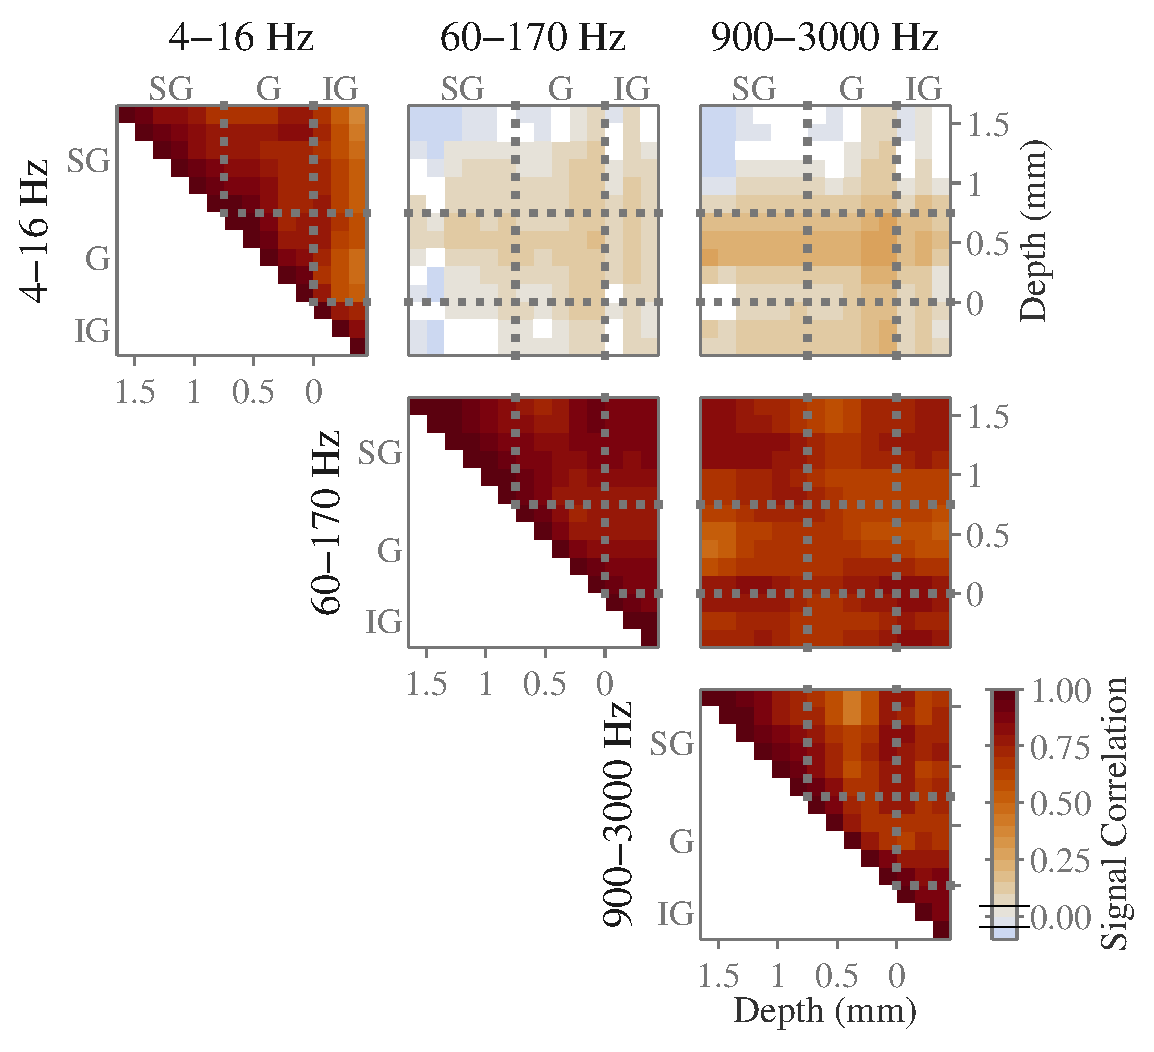
\includegraphics[scale=.34]{%
figs/noisesigcor/bndflt3-3-signal-avg_paper.eps}}
    \hspace*{\fill}
    \\
    \hspace*{\fill}
    \subfloat[][Noise correlation.\label{fig:lam_cxchn_noisecor}]{%
        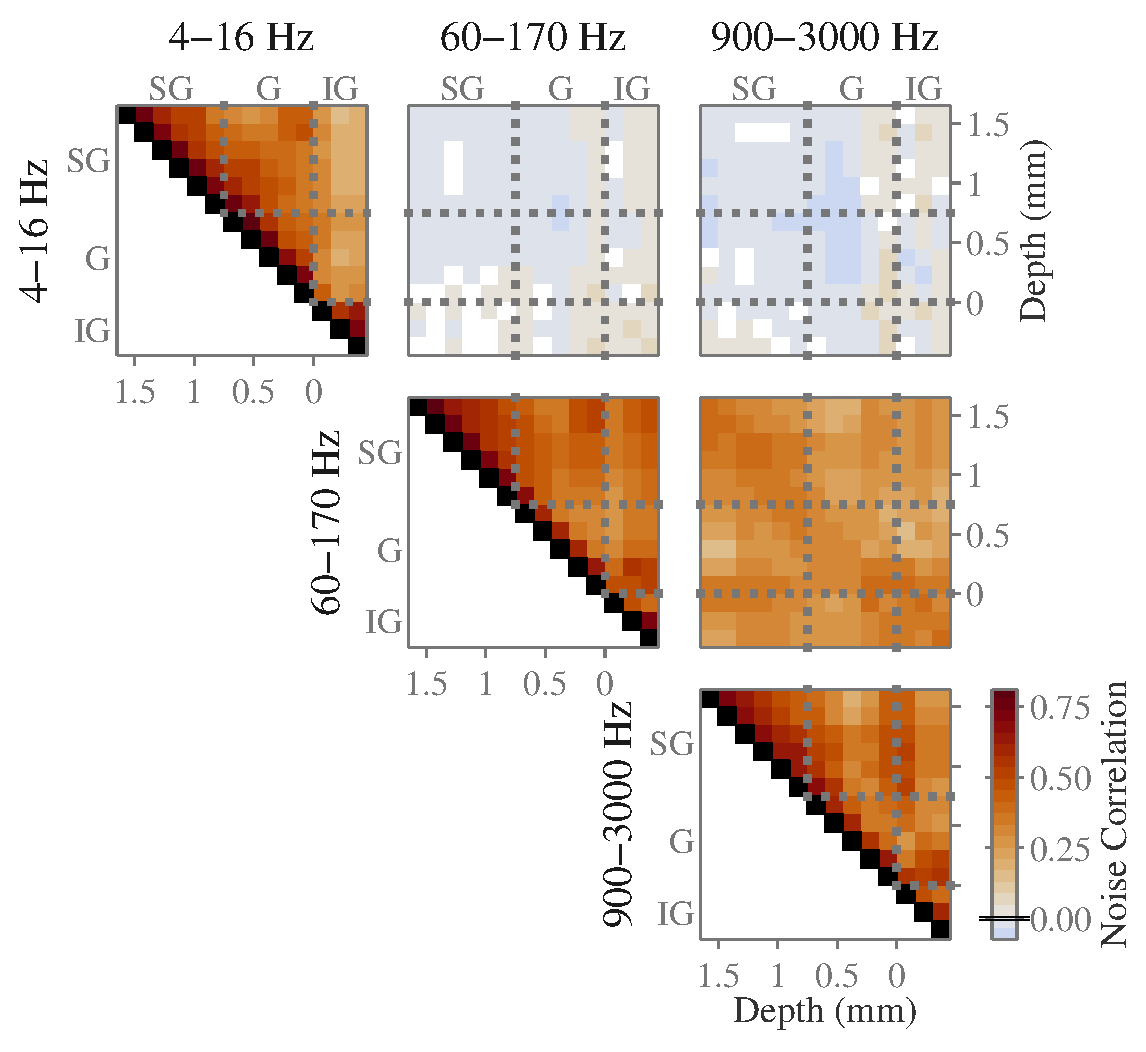
\includegraphics[scale=.34]{%
figs/noisesigcor/bndflt3-3-noise-avg_paper.eps}}
    \hspace*{\fill}
%
\caption{
\captionemph{Correlation across cortical laminae of power in \ac{CSD} frequency bands and \ac{MUA}.}
Since correlation is symmetric, the lower triangle (removed) is a mirror image of the upper triangle.
Non-significant datapoints are shown in white, with minimum and maximum significance thresholds indicated by the black lines across the colour bar.
}%
\label{fig:lam_cxchn_cor}
%
\end{figure}

These findings prompted us to investigate which properties of the stimulus were encoded by the two frequencies bands.
Since their powers contain independent information about the stimulus, we want to find two orthogonal properties of the stimulus which are encoded by these two complementary spectral bands.


\subsection{Information about scene cuts}
\label{sec:lam_scnchg}

Flash stimuli and the onset of the movie both induce large depolarisations in the cortex, with characteristic waveform profiles.
Indeed, we used the characteristic \ac{CSD} response to align our electrode penetrations between sessions (see \autoref{sec:lam_align}).
Similarly, transitions between movie scenes cause discontinuities in the content of the stimulus, which may involve a similarly large change in the gross luminance of the stimulus.
The sudden transitions associated with scene cuts can be considered analogous to the discontinuities in visual stimulation associated with saccades during natural behaviour.
Consequently, we investigated how much information the cortical response contained about scene cuts in the stimulus.

\begin{figure}[htbp]
\centering
\subfloat[][As a function the duration after the scene cut horizon threshold.\label{fig:lam_scnchg_dur}]{%
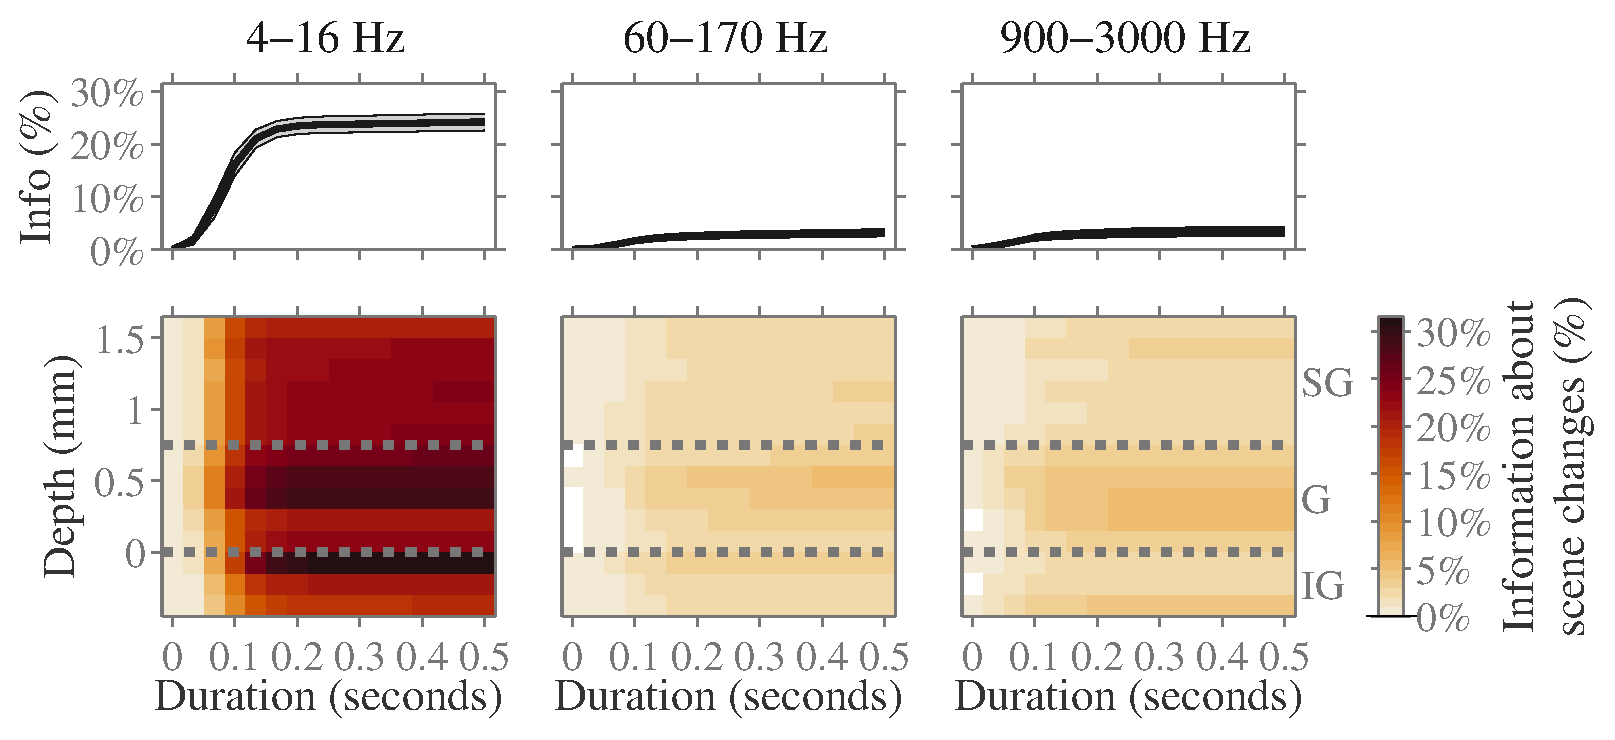
\includegraphics[scale=.375]{%
figs/scnchg/depth_v_scenecut-info_scnchg-dist_duration_avg_3.eps}}
\\
\subfloat[][Across a range of cortical frequencies.\label{fig:lam_scnchg_frq}]{%
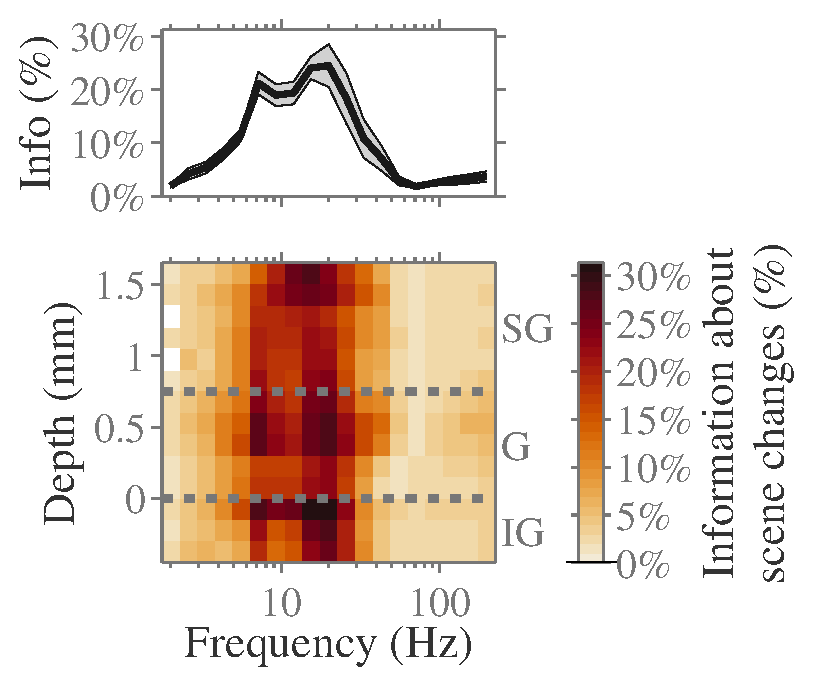
\includegraphics[scale=.375]{%
figs/scnchg/frq-power_v_depth_scenecut-info_scnchg-dist_0.200s_avg.eps}}
%
\caption{
\captionemph{Information about the presence of scene cuts.}
We computed the information about scene cuts as described in \autoref{sec:lam_scnchg_method}, and for each session expressed this as a proportion of the total information present (indicated in \autoref{fig:lam_info_sessions}) before averaging across recording sessions.
\protect\subref{fig:lam_scnchg_dur}:~Information in the power across the cortical depth for the \SIrange{4}{16}{Hz} (left) and \SIrange{60}{170}{Hz} (middle) frequency bands, and \ac{MUA} (\SIrange{900}{3000}{Hz}; right), averaged over \num{6} sessions.
Information values which were not significantly different from the bootstrap distribution are shown in white, with the median threshold for significance indicated by a black line across the colour bar.
Above, the average percentage of information explained by scene cuts over all cortical recording sites is shown, with the standard error across sessions indicated by the shaded region.
\protect\subref{fig:lam_scnchg_frq}:~Information about scene cuts contained in a range of \ac{CSD} frequencies, in which we only considered the time since the last scene cut for the \SI{0.2}{\second} immediately following each cut.
}%
\label{fig:lam_scnchg}
%
\end{figure}

This was achieved by relabelling the frames in the stimulus to encode only the length of time since the last scene cut, up to a certain threshold duration.
Information about which scene cut was presented was destroyed by ensuring the stimulus labels following each of the \num{96} scene cuts collided with each other.
Information about frames past the scene cut horizon threshold was destroyed by labelling all remaining frames as identical (see \autoref{sec:lam_scnchg_method} for more details).

We found that approximately a quarter of the information in the \SIrange{4}{16}{Hz} range pertained to the activity immediately following scene cuts, as shown in \autoref{fig:lam_scnchg_dur}.
In contrast, only about a tenth as much (\SI{2.5}{\percent}) of the information contained in both the \SIrange{60}{170}{Hz} power and the \ac{MUA} was explained by the timing of scene cuts.
Consequently, we conclude that scene changes (or saccades in natural behaviour) is one property of the visual feed which is encoded differently between the \SIrange{4}{16}{Hz} and \SIrange{60}{170}{Hz} bands.

After a short delay, due to the latency of the visual system, the amount of information about scene cuts rises and saturates quickly.
Consequently, we can conclude that \SIrange{4}{16}{Hz} power only has information about scene cuts transitively, lasting for approximately \SI{100}{\milli\second} after the response to the scene cut begins.
Also noteworthy, the fraction of the \SIrange{4}{16}{Hz} information which is about scene changes is not homogeneous: \SI{5}{\percent} to \SI{10}{\percent} more of the information encoded in upper-\ac{G} and upper-\ac{IG} was explained by scene cuts than in lower-\ac{G} and lower-\ac{IG}.
% This is agrees with previous studies showing that [CITE]

Using a static scene cut horizon of \SI{200}{\milli\second}, we investigated the fraction of information explained by scene cuts in the cortical power as a function of frequency (see \autoref{fig:lam_scnchg_frq}).
The amount of information explained by scene cuts is highest for the \SIrange{7}{20}{Hz} range.

These results demonstrate one property of the movie stimulus which is strongly encoded by one frequency range --- namely the fast, global, changes in luminance associated with scene cuts.
Next we generalised this property to consider different spatial and then temporal scales of change in the movie.


\subsection{Information about spatial frequency components of visual stimulus}

We next considered the amount of information about different spatial scales of the movie stimulus.
Since neurons in the primary visual cortex are known to respond strongly to moving sinusoidal gratings with specific spatial frequencies, it is intuitive to consider how much information the frequency bands contained about changes in luminance as a function of spatial frequency.

We decomposed the series of frames in the movie into set of spatial frequency components by finding the rate of change of luminance within a given set of spatial frequency bands (as described in \autoref{sec:lam_spares_method} and \autoref{fig:lam_spares_method}), and then computed the amount of information about this series contained in the neural activity.

\begin{figure}[htbp]
    \centering
    \hspace*{\fill}
    \subfloat[][Information about spatial components.\label{fig:lam_spares_lines}]{%
        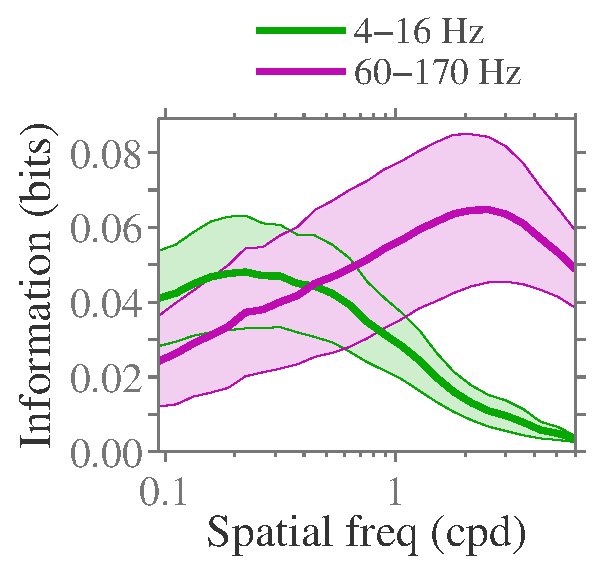
\includegraphics[scale=.34]{%
figs/spares/spares-none-linebound-logx-doLabels-region_2.eps}}
    \hspace*{\fill}\hspace{.2cm}\hspace*{\fill}
    \subfloat[][Information about spatial components in different neural frequency bands.\label{fig:lam_spares_csdfrq}]{%
        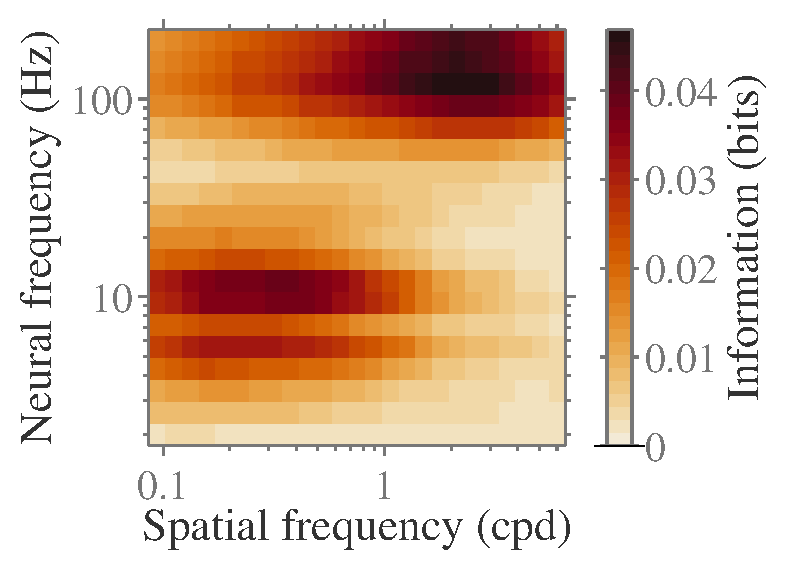
\includegraphics[scale=.34]{%
figs/spares/fig8v2-power-bands-spares-none-logx-avg-doLabels.eps}}
    \hspace*{\fill}
    \\
    \hspace*{\fill}
    \subfloat[][Information about spatial components in \SIrange{4}{16}{Hz} \acs{CSD} across cortical depth.\label{fig:lam_spares_alpha}]{%
        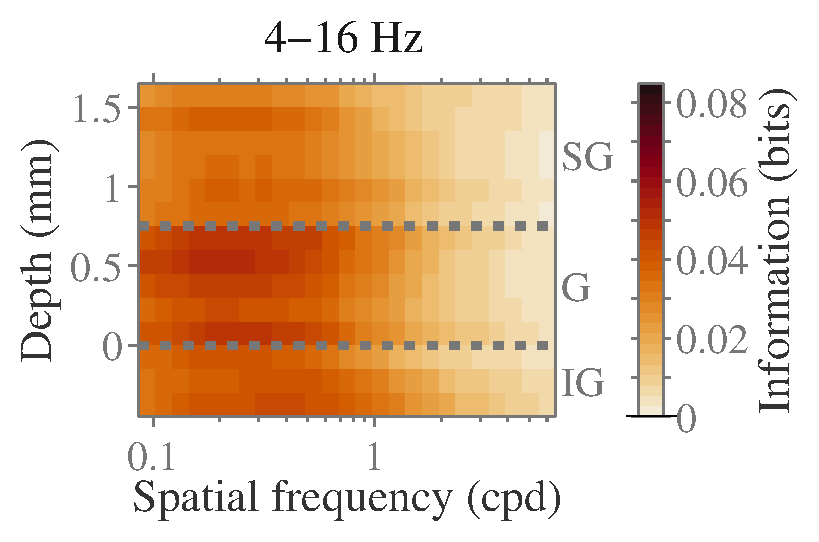
\includegraphics[scale=.34]{%
figs/spares/spares-none-logx-avg-doLabels_4-16Hz_power.eps}}
    \hspace*{\fill}\hspace{.2cm}\hspace*{\fill}
    \subfloat[][Information about spatial components in \SIrange{60}{170}{Hz} \acs{CSD} across cortical depth.\label{fig:lam_spares_gamma}]{%
        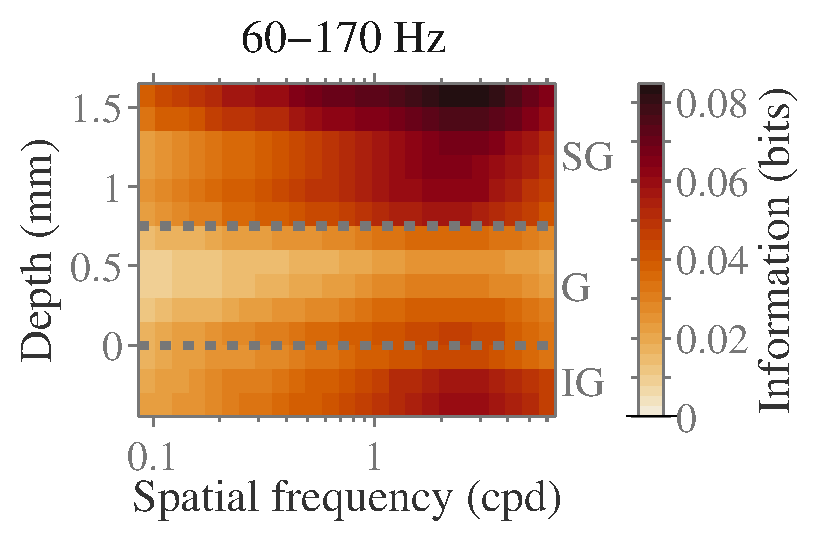
\includegraphics[scale=.34]{%
figs/spares/spares-none-logx-avg-doLabels_60-170Hz_power.eps}}
    \hspace*{\fill}
%
\caption{
\captionemph{Information about different spatial components across laminae and frequency bands.}
\protect\subref{fig:lam_spares_lines}:~Information about spatial components of the stimulus contained in low frequency \ac{CSD} power (\SIrange{4}{16}{Hz}, average of information within \ac{G} compartment; green) and high frequency \ac{CSD} power (\SIrange{60}{170}{Hz}, average of information within \ac{SG} compartment; purple).
Shaded area: standard error across \num{6} sessions.
\protect\subref{fig:lam_spares_csdfrq}:~Information about visual spatial components contained in a range of \ac{CSD} frequencies, median over \num{12} recording sites.
\protect\subref{fig:lam_spares_alpha} and \protect\subref{fig:lam_spares_gamma}:~Information in low (\SIrange{4}{16}{Hz}) and high (\SIrange{60}{170}{Hz}) \ac{CSD} frequency bands across cortical laminae.
In each plot, the mean over \num{6} sessions is indicated.
}%
\label{fig:lam_spares}
%
\end{figure}

The results are summarised in \autoref{fig:lam_spares_lines}, which shows the information encoded in the two frequency bands, averaged across the whole cortical depth.
We found the low frequency \ac{CSD} bands (\SI{<40}{Hz}) contained more information about low spatial frequencies (\SIrange{0.1}{0.6}{\cpd}), whereas the higher spectral frequencies (\SI{>40}{Hz}) contained more information about high spatial frequencies (\SIrange{0.6}{5.0}{\cpd}) (\autoref{fig:lam_spares_csdfrq}).
Importantly, there was no continuous transition between these two; instead we observe an abrupt change at \SI{40}{Hz}, with lower and higher neural oscillation frequencies tuned to stimulus features with different spatial frequencies.
Neural oscillations at intermediate frequencies do not encode intermediate spatial components of the stimulus --- they do not encode any spatial aspect of the stimulus.

These observations held true across the entire cortical depth (\autoref{fig:lam_spares_alpha} and \autoref{fig:lam_spares_gamma}), with the two frequency bands (\SIrange{4}{16}{Hz} and \SIrange{60}{170}{Hz}) containing information about opposing spatial frequencies.
% The distribution of information across the cortical depth corresponds to that found in \autoref{fig:lam_info_csd}.

Since information theoretic measures capture any possible relationship between stimulus and response, we cannot use it to determine the nature of how changes in luminance lead to changes in cortical power.
To resolve this question, we investigated the correlation between the \ac{CSD} power and both coarse (\SI{<0.3}{\cpd}, low-pass spatial filter) and fine (\SI{>1}{\cpd}, high-pass spatial filter) spatial components of the movie stimulus, illustrative example traces of which are shown above \autoref{fig:lam_6}.
These two spatial components have a relatively low coefficient of correlation with each other ($r=0.18$), indicating that although these aspects of the movie stimulus do covary, most of their behaviour is independent.

\begin{figure}[htbp]
\centering 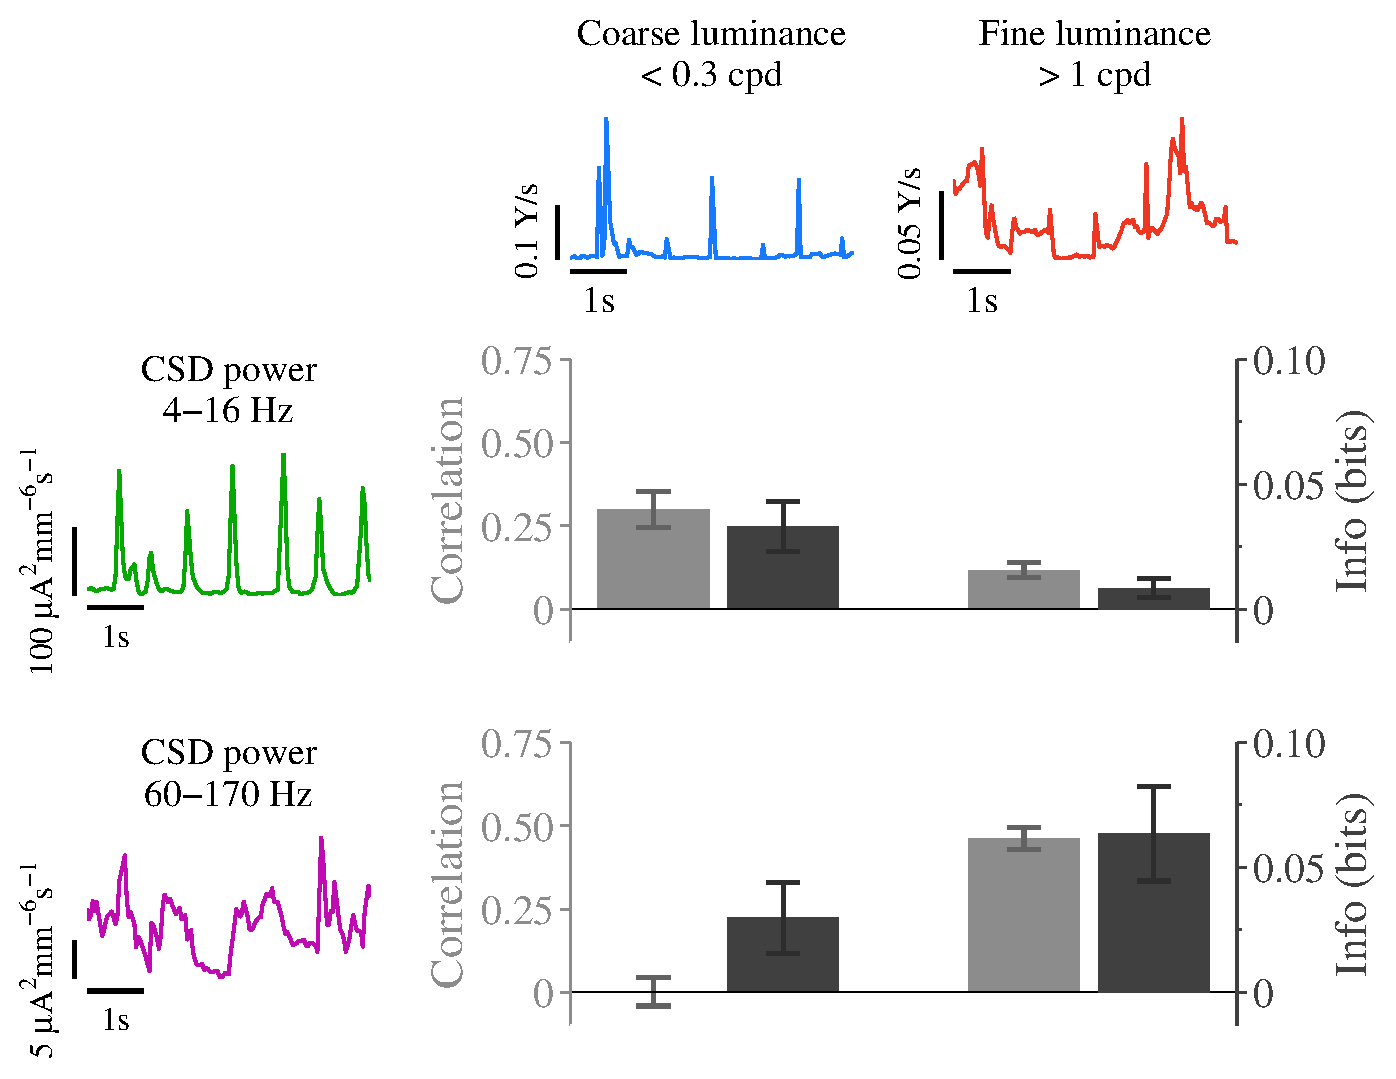
\includegraphics[scale=.4]{paperfigs/fig6A.eps}
%
\caption{
\captionemph{Overview of information components.}
Relationship between Coarse/Fine changes in luminance and Low/High frequency neural activity.
Left: Instantaneous power in \SIrange{4}{16}{Hz} band (averaged over trials and \ac{SG} layers) and \SIrange{60}{170}{Hz} band (averaged over trials and \ac{G} layers) for an example session (\sesname{H05nm7}).
Above: Coarse (\SI{<0.3}{\cpd}) and fine (\SI{>1}{\cpd}) rate of change in luminance over the same time period.
The barchart shows, for each pair of stimulus and response, Pearson's correlation coefficient (pale grey; left-hand axis) and mutual information (dark grey; right-hand axis).
}%
\label{fig:lam_6}
%
\end{figure}

We found (\autoref{fig:lam_6}) the low frequency \ac{CSD} power is positively correlated with the coarse changes in luminance, and high frequency \ac{CSD} power is positively correlated with the finer changes in luminance --- in both cases an increase in luminance of the stimulus yields an increase in power as a response.
Example \ac{CSD} traces are shown for two electrode contacts (\autoref{fig:lam_6}, left side) over same time period as the luminance example traces.
By visual inspection, one can observe that peaks and troughs in the luminance signals are coincident with peaks and troughs in the \ac{CSD} power of the appropriate frequency range.


\subsection{Information latency}

We also investigated the latency at which information about the movie was expressed across the cortical depth.
To do so, we measured the amount of information about fine and coarse changes in luminance encoded in the \ac{CSD} power, whilst varying assumed lag between stimulus and response.
The latency between stimulus and response was defined as the lag which optimised their mutual information (see \autoref{sec:lam_latency_method} for details).

Then, for each session, we compared the latency pairwise between different depths \autoref{fig:lam_latencydiff}.
We checked whether the difference in latency was consistent across sessions.
We found there was no consistent pattern to the latency between the power of \SIrange{60}{170}{Hz} oscillations with respect to changes in luminance in the \SI{>1.0}{cpd} range.
However, there was a reliable difference in latency for the information in the \SIrange{4}{16}{Hz} power (with respect to coarse changes in luminance, \SI{<0.3}{cpd}).
The channels within the \ac{G} compartment consistently had the shortest response latency, with a lead of \SI{10}{\milli\second} over \ac{SG} and upper \ac{IG} (\acs{L5}).

% Max for   4.00 -   16.00Hz,  0.000-0.300cpd is 0.0460 at 0.09850 sec
% Max for   4.00 -   16.00Hz,    1.000-Infcpd is 0.0083 at 0.07085 sec
% Max for  60.00 -  170.00Hz,  0.000-0.300cpd is 0.0121 at 0.09850 sec
% Max for  60.00 -  170.00Hz,    1.000-Infcpd is 0.0713 at 0.11578 sec
% Max for 900.00 - 3000.00Hz,  0.000-0.300cpd is 0.0411 at 0.04838 sec
% Max for 900.00 - 3000.00Hz,    1.000-Infcpd is 0.0960 at 0.08467 sec

% Lag between information in  G and IG for low2 power  0.000-0.300cpd is +0.0134+/-0.0044 seconds, p=0.0282
% Lag between information in  G and SG for low2 power  0.000-0.300cpd is +0.0089+/-0.0024 seconds, p=0.0141
% Lag between information in SG and IG for low2 power  0.000-0.300cpd is +0.0045+/-0.0050 seconds, p=0.4042
%
% Lag between information in  G and IG for low2 power    1.000-Infcpd is +0.0347+/-0.0319 seconds, p=0.3260
% Lag between information in  G and SG for low2 power    1.000-Infcpd is +0.0247+/-0.0080 seconds, p=0.0272
% Lag between information in SG and IG for low2 power    1.000-Infcpd is +0.0100+/-0.0313 seconds, p=0.7613
%
% Lag between information in  G and IG for hgh4 power  0.000-0.300cpd is -0.0114+/-0.0156 seconds, p=0.4978
% Lag between information in  G and SG for hgh4 power  0.000-0.300cpd is +0.0063+/-0.0052 seconds, p=0.2789
% Lag between information in SG and IG for hgh4 power  0.000-0.300cpd is -0.0177+/-0.0183 seconds, p=0.3775
%
% Lag between information in  G and IG for hgh4 power    1.000-Infcpd is -0.0092+/-0.0095 seconds, p=0.3779
% Lag between information in  G and SG for hgh4 power    1.000-Infcpd is +0.0011+/-0.0067 seconds, p=0.8781
% Lag between information in SG and IG for hgh4 power    1.000-Infcpd is -0.0103+/-0.0067 seconds, p=0.1837
%
% Lag between information in  G and IG for  mua power  0.000-0.300cpd is -0.0048+/-0.0105 seconds, p=0.6685
% Lag between information in  G and SG for  mua power  0.000-0.300cpd is -0.0056+/-0.0124 seconds, p=0.6697
% Lag between information in SG and IG for  mua power  0.000-0.300cpd is +0.0009+/-0.0057 seconds, p=0.8857
%
% Lag between information in  G and IG for  mua power    1.000-Infcpd is +0.0009+/-0.0027 seconds, p=0.7646
% Lag between information in  G and SG for  mua power    1.000-Infcpd is -0.0048+/-0.0033 seconds, p=0.2024
% Lag between information in SG and IG for  mua power    1.000-Infcpd is +0.0057+/-0.0030 seconds, p=0.1193

\begin{figure}[htbp]
\centerline{
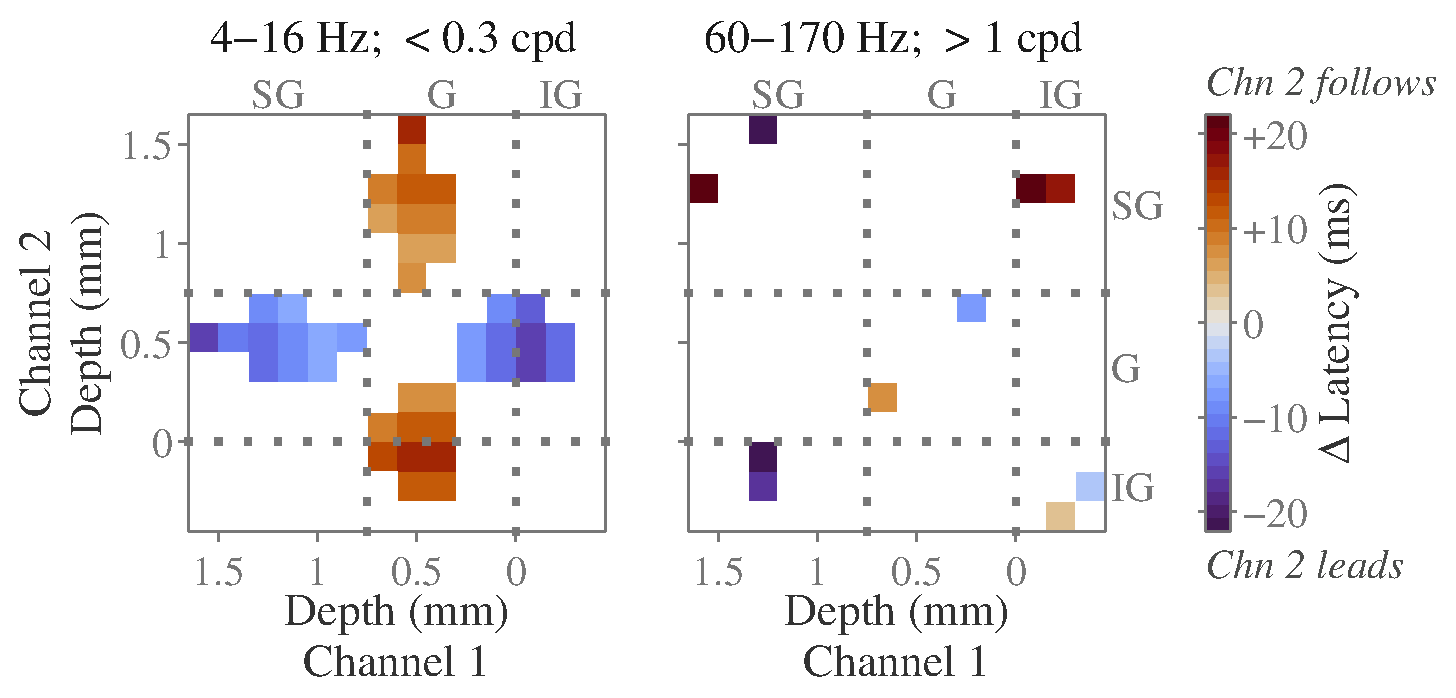
\includegraphics[scale=.375]{figs/lag/latencydifference-avg_nonsig1.eps}
}
%
\caption{
\captionemph{Difference in peak information latency between recording depths.}
We present the difference in latency between pairs of recording channels, from Channel 1 to Channel 2; if $\Delta$ is positive, Channel 1 precedes Channel 2.
Left: difference in the latency of peak information between channels, for information about coarse luminance changes (\SI{<0.3}{cpd}) encoded in the power of \SIrange{4}{16}{Hz} oscillations.
Right: information in the \SIrange{60}{170}{Hz} power range about finer scaled, \SI{>1.0}{cpd}, luminance changes.
Both plots show the average over \num{6} sessions, with non-significant differences in latency (Student's $t$-test) shown in white.
}
\label{fig:lam_latencydiff}
\end{figure}


\subsection{Information about spatio-temporal components of visual stimulus}
\label{sec:lam_spatmf}

Next, we considered the information about different temporal components of the movie.
We extracted specific temporal frequency bands of the luminance signal in the movie using the same method as the spatial components, but with a temporal filter after taking the derivative of the spatially filtered luminance (see \autoref{sec:lam_tmf_method} for more details).

\begin{figure}[htbp]
\centerline{
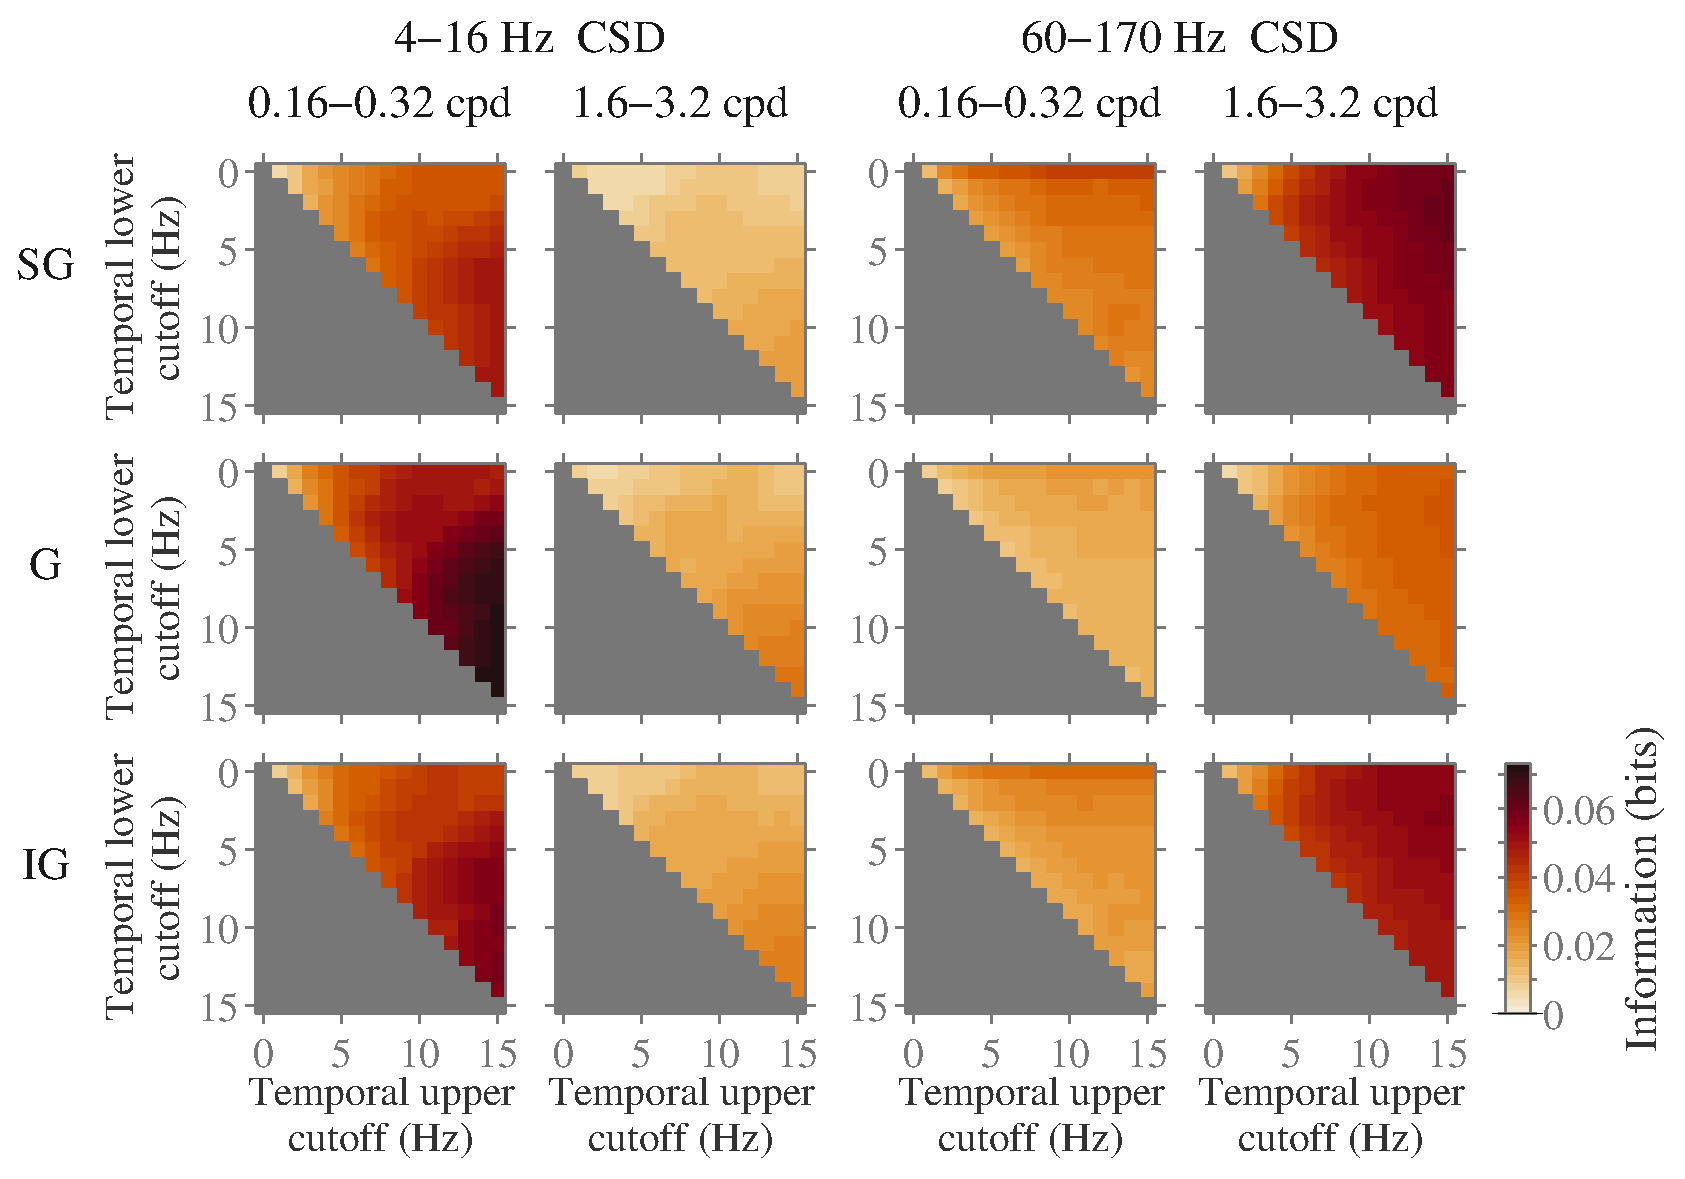
\includegraphics[scale=.375]{figs/tmf/tmf-v-tmf-sggig-avg-tmfres1b-2Band-2Crs.eps}
}
%
\caption{
\captionemph{Information about different temporal components of the stimulus.}
The amount of information about the rate of change of luminance encoded in \SIrange{4}{16}{Hz} (left two columns) and \SIrange{60}{170}{Hz} (right two columns) frequency bands of the neural \ac{CSD} activity, subject to either a low or high spatial filter (width of one octave) and a temporal filter.
We applied temporal filters (6th-order \ac{IIR} Butterworth filter) with lower cutoff $f_\text{low}$ from \num{0}{Hz} to \num{14}{Hz} ($y$-axes) and upper cutoff $f_\text{up}$ from $f_\text{low}$ to \num{15}{Hz} ($x$-axes).
(In the case $f_\text{low} = 0$, a lowpass filter was used instead of a bandpass.)
The lower triangle of each panel, where $f_\text{up} < f_\text{low}$, is omitted.
Each row of panels corresponds to a different cortical depth, averaging over \ac{SG}, \ac{G} and \ac{IG} compartments, respectively.
Throughout all panels, the mean over \num{6} sessions is indicated.
Statistical significance thresholds were computed for each datapoint individually, and a typical significance threshold is shown by the black line across the colour bar, near $0$.
}
\label{fig:lam_tmf}
%
\end{figure}

First, we considered two spatial frequency bands, \SIrange{0.16}{0.32}{cpd} and \SIrange{1.6}{3.2}{cpd}, each of which was one octave in width and corresponded (see \autoref{fig:lam_spares}) to the peak information in one of the two \ac{CSD} frequency bands, either \SIrange{4}{16}{Hz} or \SIrange{60}{170}{Hz}.
We extracted temporal components of these two spatial signals using a series of bandpass filters whose lower cutoff frequencies ranged linearly from \SIrange{0}{14}{Hz} and upper cutoff frequencies ranged from \SIrange{1}{15}{Hz} (the Nyquist frequency of the movie stimulus).
% Consequently the widths of the extracted frequency varied over \SI{1}{15}{Hz}.

The \SIrange{4}{16}{Hz} \ac{CSD} power contains most information about high temporal frequency components of the low spatial frequency changes in the movie (\autoref{fig:lam_tmf}, left-most column).
These components include scene cuts and similar stimuli, where there is a sudden gross change in the stimulus.
In contrast, the information about coarse, \SIrange{0.16}{0.32}{cpd}, stimuli which is encoded in the \SIrange{60}{170}{Hz} \ac{CSD} frequency range is preferentially about the slow temporal components instead of fast.
The information peaks with a lowpass filter (shown as \SI{0}{Hz} lower cutoff in \autoref{fig:lam_tmf}), indicating that the information contained in this aspect of the cortical response is closely tied to the absolute magnitude of the change in luminance.

% Though the \SIrange{4}{16}{Hz} \ac{CSD} band does not contain much information about finer-grained details (\SIrange{1.6}{3.2}{cpd} spatial band) about the movie, the information it does have is again in the high-temporal frequency range.
We had already identified that the \SIrange{60}{170}{Hz} \ac{CSD} range contained most information about the finer spatial scales in the movie.
Now we also observe that a broad range of temporal components contribute to this signal, with a peak for the \SIrange{3}{15}{Hz} temporal range of the stimulus (\autoref{fig:lam_tmf}, right-most column).


We wanted to consider the information about spatiotemporal components of the movie as a continuous function of both spatial and temporal frequency ranges.
For this, we fixed the temporal bandwidth as \SI{6}{Hz} and again fixed the spatial bandwidth as one octave.
As shown in \autoref{fig:lam_spatmf}, the two \ac{CSD} frequency ranges contain information about entirely complementary spatiotemporal components of the stimulus, and the \ac{MUA} contains information about the same spatiotemporal range as the \SIrange{60}{170}{Hz} power.

\begin{figure}[htbp]
\centerline{
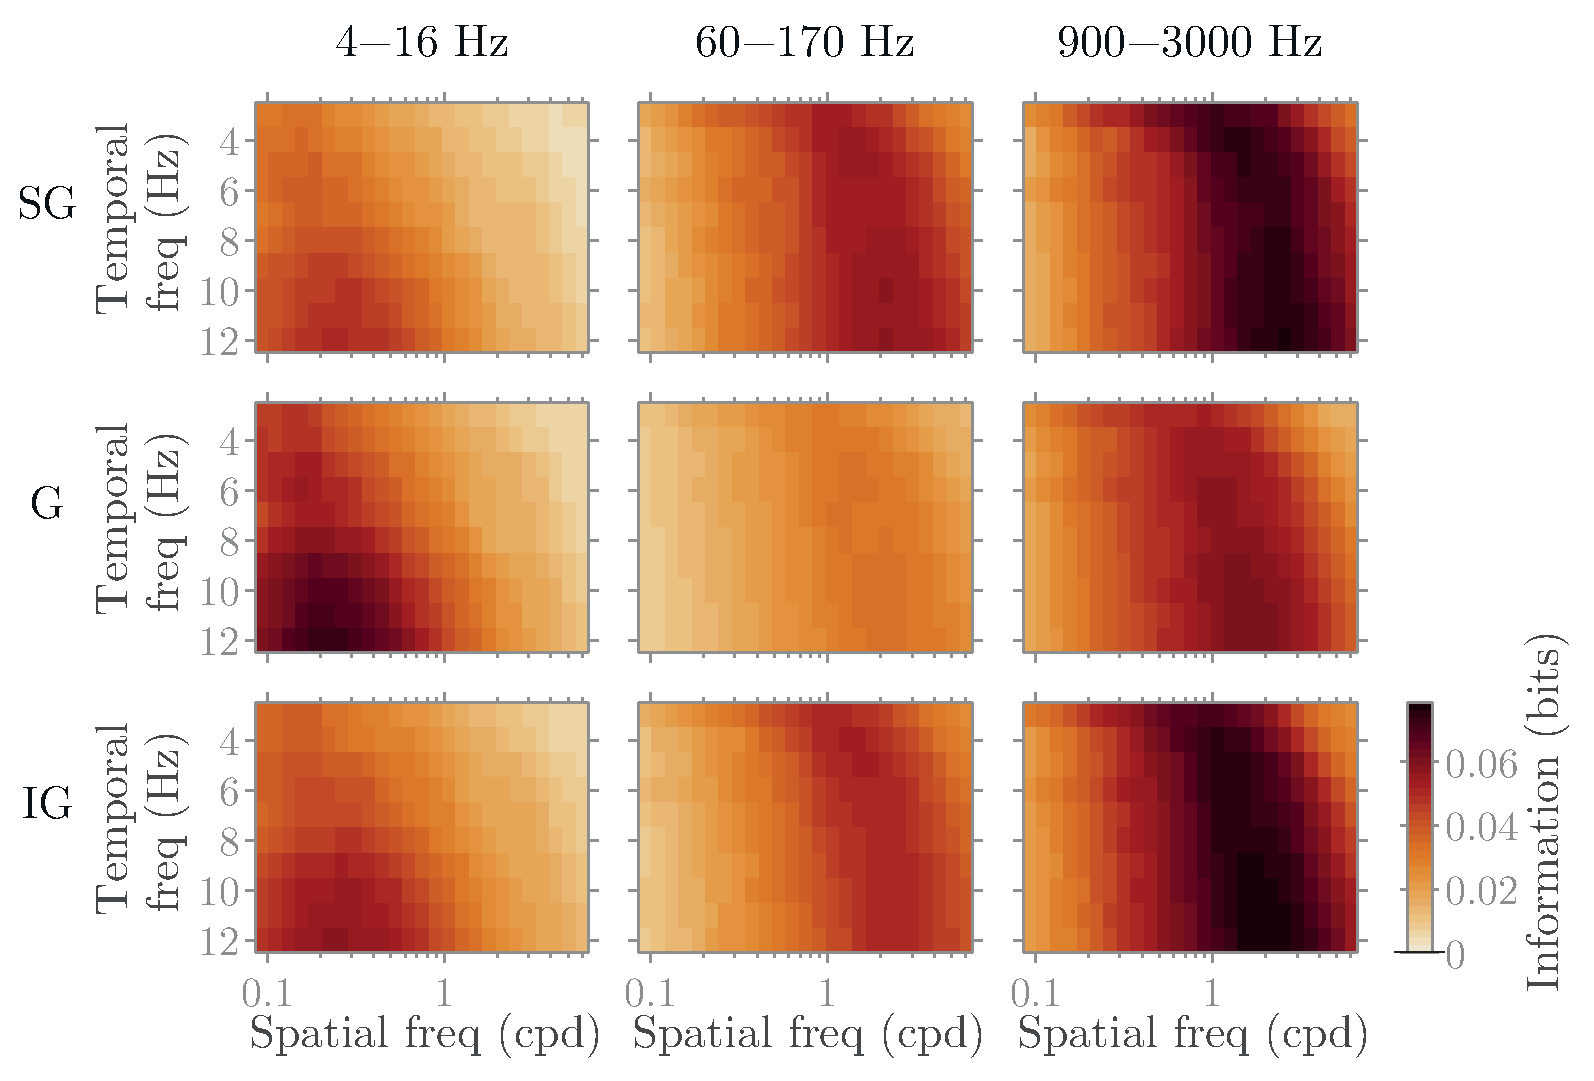
\includegraphics[scale=.375]{figs/tmf/spatmf2_3bnd.eps}
}
%
\caption{
\captionemph{Information about different spatiotemporal components.}
The luminance of the movie was filtered in the spatial domain with using bandpass filters each with width one octave, and in the temporal domain with bandpass filters each with width \SI{6}{Hz}.
Datapoints are shown against the middle of the band on both $x$ and $y$ axes.
We show the amount of information about the rate of change of filtered luminance encoded in the \SIrange{4}{16}{Hz} frequency range of the \ac{CSD} (left column), information in \SIrange{60}{170}{Hz} power (middle), and information in the \ac{MUA} (right).
Each row of panels corresponds to a different cortical depth, averaging over \ac{SG}, \ac{G} and \ac{IG} compartments, respectively.
Throughout all panels, the mean over \num{6} sessions is indicated.
Statistical significance thresholds were computed for each datapoint individually, and a typical significance threshold is shown by the black line across the colour bar, near $0$.
}%
\label{fig:lam_spatmf}
%
\end{figure}


% =============================================================================
\section{Conclusions}
\label{sec:lam_discussion}
% =============================================================================

In summary, we find that while the average power of cortical oscillations is distributed similarly across the entire cortical depth, the strength of these oscillations at particular frequencies are tuned to the stimulus at certain depths (\autoref{fig:lam_info}).
Previous work by \citet{Belitski2008} demonstrated there are two cortical frequency bands (\SI{<40}{Hz} and \SI{>40}{Hz}) within \ac{V1} which encode independent information about the natural visual scenes.
We discovered that these frequency bands are partially redundant within themselves across the whole cortical depth, but the information contained within them is localised at specific cortical laminae.
In particular, the \SIrange{4}{16}{Hz} frequency band is informative in the upper granular and mid-infragranular compartments, and the \SIrange{60}{170}{Hz} range at upper supragranular and mid-infragranular regions.

We investigated which unique properties of the stimulus may be encoded by each frequency band.
The occurrence of scene cuts in the movie, whose effects can be considered analogous to saccades in natural behaviour, accounted for a quarter of the information in the \SIrange{7}{20}{Hz} band, but a negligible fraction of the information present in other frequencies.

Subsequently, we examined whether changes in luminance at different spatial frequencies induced differential changes in the cortex as a function of neural frequency and depth.
In corroboration with the results for scene cuts, we found that a similar frequency range, \SIrange{4}{16}{Hz}, encoded information about changes in the low spatial frequency aspects of the stimulus.
The high frequency components of the neural activity, \SI{>60}{Hz}, encoded information about the high spatial frequency components of the stimulus, shown in \autoref{fig:lam_spares_csdfrq}.

Extending our decomposition of the natural stimulus into the temporal domain, we found our two neural frequency bands encoded information about different spatiotemporal aspects of the stimulus.
The \SIrange{4}{16}{Hz} band of neural oscillations conveyed most information about sudden, coarse, changes in the stimulus --- such as would be induced by scene transitions in the movie presented and saccades in natural behaviour.
The \SIrange{60}{170}{Hz} band of neural activity conveyed information about complementary spatiotemporal components at higher spatial frequency spanning across all temporal ranges.
The peak spatial range encoded by this band was dependent on the temporal frequency range considered, with shorter temporal frequencies corresponding to broader changes in the stimulus.

Our results suggest there is multiplexing in the cortex, with low frequency and high frequency oscillations of the same population activity simultaneously encoding low and high spatial frequency components of the stimulus respectively.
This finding corroborates previous results studying \ac{EEG}: \citet{Smith2006} found that two bands of oscillations --- theta (\SIrange{4}{8}{Hz}) and beta (\SIrange{12}{25}{Hz}) --- correspond to the conscious perception of low and high spatial frequency aspects (respectively) of a bistable image.

As \ac{L4} is generally regarded as the principal layer of \ac{V1} receiving afferent inputs from the \ac{LGN} (see \autoref{sec:bg_v1}; \citealp{Callaway1998,Horton2005,Nassi2009,Harris2013}), this begs the question of how information in the gamma band has ``arisen'' in \ac{SG} layers without passing through \ac{G}.
Of course, since axons from the \ac{LGN} target specific sites within \ac{L4} of \ac{V1}, it is reasonable to assume that fine-resolution information about the visual stimulus arrives from the \ac{LGN} into \ac{L4} of \ac{V1}, with the information encoded in the pattern of \ac{V1} neurons activated by these afferent connections.
Such information is not detectable from the population level activity.
From there, fine-scale information can be redirected to \ac{SG}, where it is encoded in oscillations of activity in the \SIrange{60}{170}{Hz}.

As we discussed in \autoref{sec:bg_visual_system}, the most important visual pathways from the retina to \ac{V1} are the P- and M-pathways.
The M-pathway is encoded by parasol ganglion cells in the retina, which are responsive to low spatial and high temporal frequencies.
This pathway terminates in \ac{L4Ca} of \ac{V1}.
The P-pathway originates with midget ganglion cells, encoding low temporal, high spatial frequencies of the stimulus and terminating in \acsu{L4Cb} of \ac{V1}.

The properties of these two pathways are reminiscent of properties of the two frequency bands we have isolated.
The \SIrange{4}{16}{Hz} power pertains to changes in the stimulus with high temporal, low spatial frequencies, like the parasol ganglion cells.
The \SIrange{60}{170}{Hz} power and \ac{MUA} pertain to changes in the stimulus with high spatial frequencies, similar to the midget ganglion cells.
Consequently, these frequency bands in \ac{V1} may be conveying information passed directly through the M- and P-pathways from the retina.
The information could, hypothetically, be encoded into these frequency ranges by the \ac{LGN}, or within \ac{V1}.

The terminus locations for the M- and P-pathways are mid- and lower-\ac{G}, which is not the cortical depths for which we identified the origins of the two informative frequency bands.
However, this does not disprove the hypothesis, since the dendritic and somatic structures of the cortical neurons in \ac{V1} are spatially extended, spanning multiple layers.
Even if the feedforward visual information from \ac{LGN} solely terminated in the \ac{G} compartment (which it does not), the information could be transferred to other cortical depths before oscillatory population activity is generated.

There are several other possible interpretations of our findings.
For instance, the segregation of visual information into two frequency bands may be preparation for the fork in the visual hierarchy into dorsal (motion-sensitive) and ventral (shape-sensitive) streams.
It has previously been hypothesised that the M-pathway steered information to the dorsal stream and the P-pathway to the ventral stream.
Studies since have demonstrated that activity in \ac{MT} is dependent on both M- and P-pathways \citep{Merigan1991,Yabuta2001}.
Our results may be indicative of two different pathways for transmission of information between cortices, in which \ac{V1} integrates both M- and P-pathways together and then separates them out again.
However, this seems like an ambitious objective for \ac{V1} to achieve.

As discussed in \autoref{sec:bg_v1}, neurons in \ac{V1} are known to be tuned to the orientation, spatial frequency, direction of motion, and colour of oriented bars.
Functionally, this is similar to edge detection, which requires high spatial frequency contrast in the stimulus.
It is therefore possible that the \SIrange{60}{170}{Hz} power reflects the output of the cortical column.
Such a hypothesis could be tested by investigating whether cortical power in this frequency range is tuned to orientated bar stimuli.

The information encoded in the \SIrange{4}{16}{Hz} power pertained to coarse, sudden changes in the stimulus, such as scene cuts.
When coarse and fast changes occur in the movie, the next frame seen by the cortex is very different from the previous stimuli in an unpredictable manner.
Should \ac{V1} be utilising predictive coding, a sudden change in the stimulus such as this would violate the expected input predicted by \ac{V1}.
Consequently, it may be that \SIrange{4}{16}{Hz} activity reflects an error signal, either triggering the latent state of \ac{V1} neurons to correct for the error or reset ready for a new initialisation.

Recent work has shown that stimulation in \ac{V1} induces gamma (\SIrange{40}{90}{Hz}) activity in \ac{V4} (feedforward), whilst stimulation in \ac{V4} induces alpha (\SIrange{5}{15}{Hz}) oscillations in \ac{V1} (feedback) \citep{VanKerkoerle2014}.
These results seem to lend further credence to the interpretation of alpha as a feedback error signal and gamma as a feedforward output of \ac{V1}.
\citet{VanKerkoerle2014} also found that the gamma waves were initiated at \ac{L4}, propagating outwards to the top of \ac{SG} and bottom of \ac{IG}.
Alpha waves propagated in the opposite direction, originating at the top and bottom of the cortex and travelling the middle.
Our own analysis demonstrated that the gamma band was most informative at the top and bottom boundaries of the cortical column, and alpha in the middle of \ac{L4}.
These localisations are the terminus of the \citet{VanKerkoerle2014} waves, not their origins as we would have initially expected.
Reconciling these results together, we hypothesise that the cortical waves are gated as they travel through the cortical depth, such that the amplitude of the oscillations is amplified and supressed in a stimulus-dependent manner.
However, this is a complex interpretation of the data and more evidence is needed to test its validity.

We discuss possible future work to resolve these issues and questions in \autoref{ch:discussion}.
